% !TEX root = ../enac_project_fr.tex
%%%%%%%%%%%%%%%%%%%%%%%%%%%%%%%%%%%%%%%%%%%%%%%%%%%%%%%%%%%%%%%%%%%%
% Chapter 6 - Résultats et validation
%%%%%%%%%%%%%%%%%%%%%%%%%%%%%%%%%%%%%%%%%%%%%%%%%%%%%%%%%%%%%%%%%%%%

\chapter{Résultats et validation}
\label{resultats_validation}

Ce chapitre évalue les solutions produites par l'application Java--Orekit et
les compare à celles d'un logiciel indépendant. Deux propriétés sont
distinguées. La \emph{fidélité de reproduction} mesure la proximité entre les
résultats Java--Orekit et RTKLIB pour une même configuration. L'\emph{exactitude}
mesure, quant à elle, l'écart de chaque solution à la position connue de la
station. Deux traitements peuvent donc être proches l'un de l'autre tout en
présentant un biais commun, ou atteindre une exactitude comparable par des
trajectoires de convergence différentes.


\section{Logiciel de référence}
\label{sec:rtklib_reference}

RTKLIB est un ensemble logiciel libre consacré au positionnement GNSS standard
et précis. Il fournit notamment des traitements ponctuels, différentiels et
PPP, en temps réel ou en post-traitement, ainsi que les lecteurs des principaux
formats GNSS~\cite{rtklib_manual_242}. Son code source et ses fichiers de
configuration rendent explicites les modèles activés, ce qui permet de
construire des essais à paramètres identiques.

RTKLIB constitue l'unique logiciel externe retenu dans ce travail pour la
validation croisée du positionnement. Il ne fournit pas une vérité terrain :
la position de référence de la station remplit ce rôle. RTKLIB sert à vérifier
qu'une chaîne de calcul indépendante, soumise aux mêmes données et aux mêmes
hypothèses, produit une solution comparable.

Deux modes de RTKLIB sont principalement utilisés :

\begin{itemize}
    \item le mode \emph{Single} traite uniquement le code par moindres carrés
    pondérés. La correction ionosphérique est obtenue au choix par le modèle de
    Klobuchar ou par la combinaison iono-free, tandis que la troposphère
    est corrigée par le modèle de Saastamoinen. Les éphémérides sont diffusées
    et les corrections fines associées au traitement de phase ne sont pas
    activées. L'erreur observée est de l'ordre du mètre dans le plan horizontal
    et de quelques mètres en trois dimensions ;

    \item le mode \emph{PPP Static} combine code et phase dans un filtre de
    Kalman étendu. Les essais les plus complets utilisent la combinaison
    iono-free, l'estimation du ZTD et de ses gradients, les orbites et
    horloges précises, les biais de code et de phase, les marées solides, les
    corrections d'antenne et le wind-up. Après convergence, l'erreur devient
    centimétrique dans le plan horizontal et reste inférieure au décimètre en
    trois dimensions pour le cas présenté dans ce chapitre.
\end{itemize}

Dans les deux modes, les constellations GPS seule ou GPS et Galileo peuvent
être sélectionnées.


\section{Protocole de comparaison}
\label{sec:validation_protocol}

\subsection{Définition d'une configuration}

Une exécution est définie par les choix indépendants suivants, sous réserve de
leur cohérence physique :

\begin{itemize}
    \item les observables : code seul ou code et phase ;
    \item la correction ionosphérique : modèle de Klobuchar (KLO) ou
    combinaison iono-free (IF) ;
    \item le traitement troposphérique : Saastamoinen (SAAS), estimation du
    ZTD, ou estimation du ZTD et des gradients horizontaux (ZTD+GRAD) ;
    \item les éphémérides : diffusées (BROADCAST) ou précises (PRECISE) lorsque
    la phase est traitée ;
    \item les constellations : GPS ou GPS+Galileo ;
    \item le jour de l'année : 090 ou 137 ;
    \item la station : TLSG, située à Toulouse, ou YEBE, située à Yebes dans la
    région de Madrid.
\end{itemize}

Dans la configuration précise complète, les produits SP3, CLK et BIA sont
associés aux corrections de marées solides, de centre de phase d'antenne et de
wind-up. Ces options ne sont pas ajoutées au mode \emph{Single}, car leur
amplitude est faible devant le bruit des mesures de code.


\subsection{Configurations retenues}

La validation suit une démarche différentielle. Une configuration de référence
est d'abord définie pour le mode \emph{Single}, puis un seul paramètre est
modifié à la fois : station, constellation ou modèle ionosphérique. La même
méthode est appliquée à l'EKF : le modèle SAAS avec éphémérides diffusées sert
de référence, avant l'introduction de l'estimation troposphérique puis des
produits précis.

Les trois variantes du mode Single sont calculées à partir de S-REF. S-GAL
ajoute Galileo, S-KLO remplace la combinaison iono-free par Klobuchar et
S-YEBE remplace TLSG par YEBE. Le passage de E-GRAD à PPP modifie un bloc
cohérent plutôt qu'un paramètre isolé : les produits précis imposent
simultanément les orbites, les horloges, les biais et les corrections fines
associées.

\begin{table}[H]
\centering
\caption{Configurations représentatives utilisées dans ce chapitre.}
\label{tab:validation_cases}
\small
\setlength{\tabcolsep}{3pt}
\begin{tabularx}{\textwidth}{
    p{1.43cm} p{1.13cm} p{0.9cm} p{1.69cm} p{2.09cm}
    p{0.8cm} p{2.0cm} p{1.35cm} X}
\hline
\textbf{Cas} & \textbf{Station} & \textbf{Méth.} & \textbf{Obs.} &
\textbf{Const.} & \textbf{Iono.} & \textbf{Tropo.} &
\textbf{Éphém.} & \textbf{Réf.} \\
\hline
S-REF  & TLSG & WLS & code       & GPS         & IF  & SAAS     & diffusées & -- \\
S-YEBE & YEBE & WLS & code       & GPS         & IF  & SAAS     & diffusées & S-REF \\
S-GAL  & TLSG & WLS & code       & GPS+Galileo & IF  & SAAS     & diffusées & S-REF \\
S-KLO  & TLSG & WLS & code       & GPS         & KLO & SAAS     & diffusées & S-REF \\
E-REF  & TLSG & EKF & code+phase & GPS         & IF  & SAAS     & diffusées & -- \\
E-GRAD & TLSG & EKF & code+phase & GPS         & IF  & ZTD+GRAD & diffusées & E-REF \\
PPP    & TLSG & EKF & code+phase & GPS         & IF  & ZTD+GRAD & précises  & E-GRAD \\
\hline
\end{tabularx}
\end{table}

\subsection{Indicateurs}

Pour chaque époque $k$, la position estimée est comparée à la position connue
de la station dans le repère local Est--Nord--Vertical. Les erreurs horizontale
et tridimensionnelle sont définies par

\begin{equation}
e_{2D,k}=\sqrt{e_{E,k}^{2}+e_{N,k}^{2}},
\qquad
e_{3D,k}=\sqrt{e_{E,k}^{2}+e_{N,k}^{2}+e_{U,k}^{2}}.
\label{eq:validation_errors}
\end{equation}

avec :

\begin{itemize}
    \item $e_{E,k}$, $e_{N,k}$ et $e_{U,k}$ les composantes de l'erreur de
    position à l'époque $k$ dans le repère local ;
    \item $e_{2D,k}$ la norme de l'erreur dans le plan horizontal ;
    \item $e_{3D,k}$ la norme de l'erreur tridimensionnelle.
\end{itemize}

La RMSE d'une grandeur $e$ sur $n$ époques vaut

\begin{equation}
\operatorname{RMSE}(e)=
\sqrt{\frac{1}{n}\sum_{k=1}^{n}e_k^2}.
\label{eq:validation_rmse}
\end{equation}

avec :

\begin{itemize}
    \item $e_k$ l'erreur considérée à l'époque $k$ ;
    \item $n$ le nombre d'époques comparées.
\end{itemize}

La différence directe
$\Delta e_k=e_k^{\mathrm{Java}}-e_k^{\mathrm{RTKLIB}}$ complète cette mesure
d'exactitude par un indicateur de fidélité. Les nuages dans le plan horizontal
permettent en outre de comparer la dispersion, les biais et la trajectoire de
convergence.

\section{Validation du mode Single}
\label{sec:validation_wls}

\subsection{Configuration de référence et changement de station}

S-REF est la configuration la plus simple considérée : code seul, WLS, GPS,
combinaison iono-free, modèle de Saastamoinen et éphémérides diffusées.
Les figures~\ref{fig:ch5_single_station} et
\ref{fig:ch5_single_station_cdf} comparent cette référence à TLSG avec le même
traitement à YEBE. Le seul paramètre modifié est donc la station.

\begin{figure}[H]
    \centering
    \begin{minipage}[t]{0.48\textwidth}
        \centering
        \textbf{S-REF : TLSG}\par\medskip
        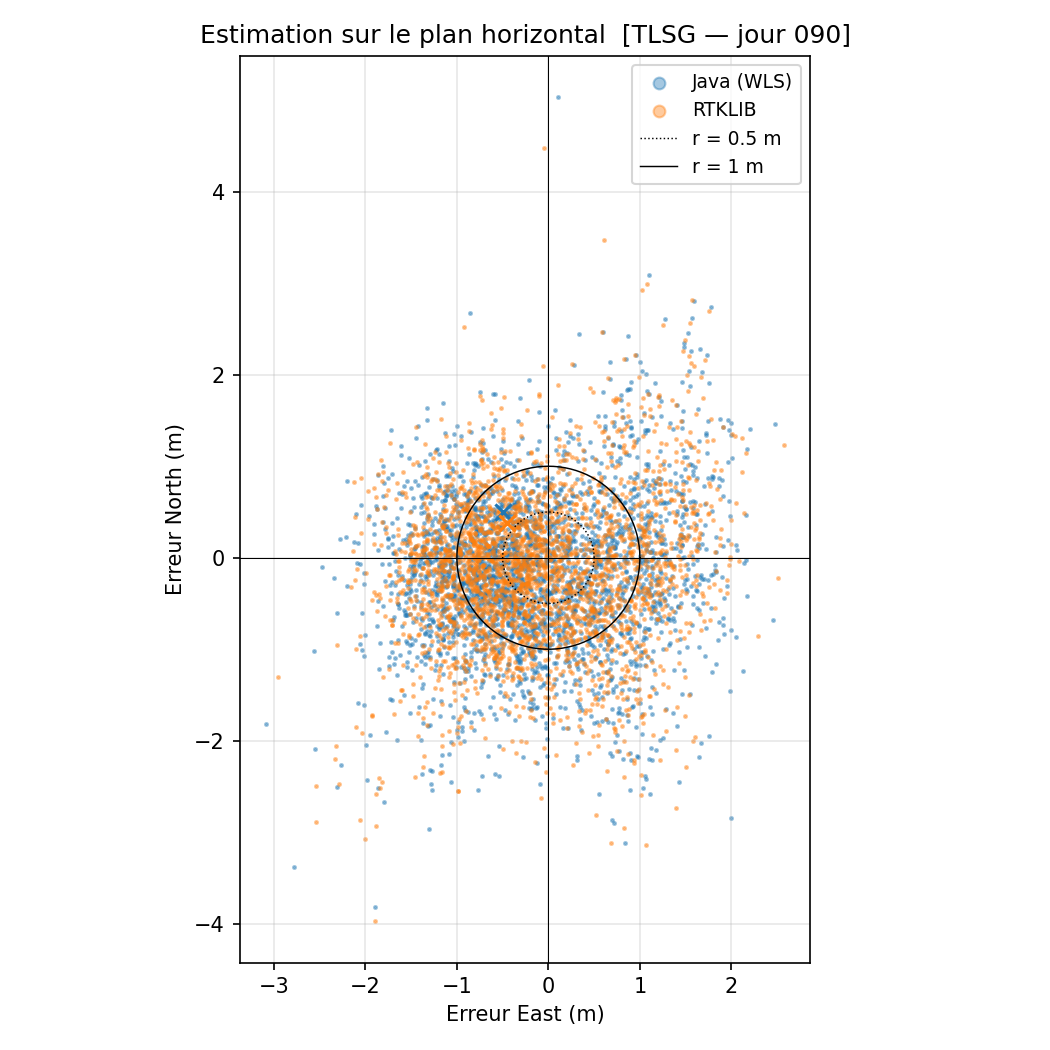
\includegraphics[width=\linewidth]{images/chapter5/ch5_wls_tlsg_j090_gps_if_saas_scatter_en.png}
    \end{minipage}
    \hfill
    \begin{minipage}[t]{0.48\textwidth}
        \centering
        \textbf{S-YEBE : YEBE}\par\medskip
        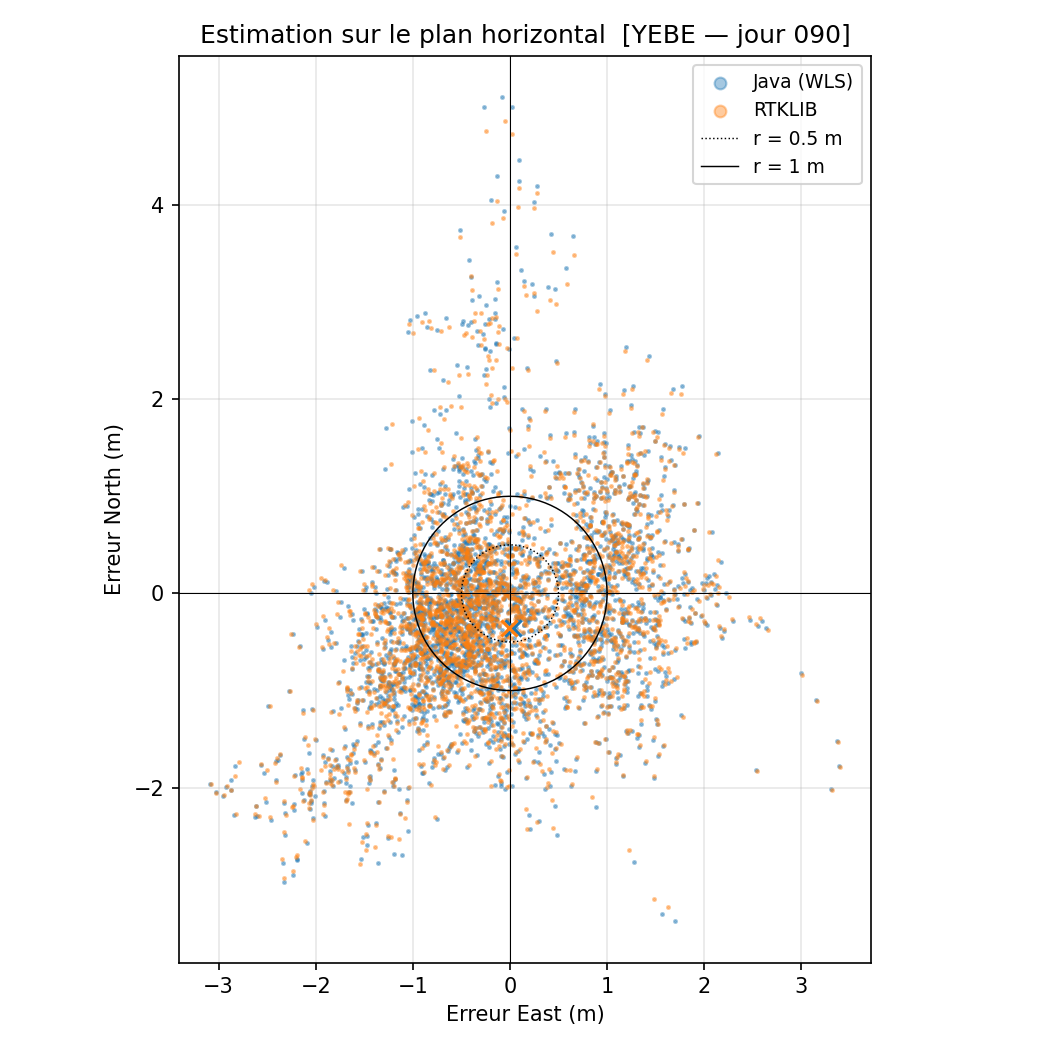
\includegraphics[width=\linewidth]{images/chapter5/ch5_wls_yebe_j090_gps_if_saas_scatter_en.png}
    \end{minipage}
    \caption{Effet du changement de station en mode Single. À gauche :
    référence S-REF ; à droite : même configuration à YEBE.}
    \label{fig:ch5_single_station}
\end{figure}

\begin{figure}[H]
    \centering
    \makebox[\textwidth][c]{%
    \begin{minipage}[t]{0.64\textwidth}
        \centering
        \textbf{S-REF : TLSG}\par\medskip
        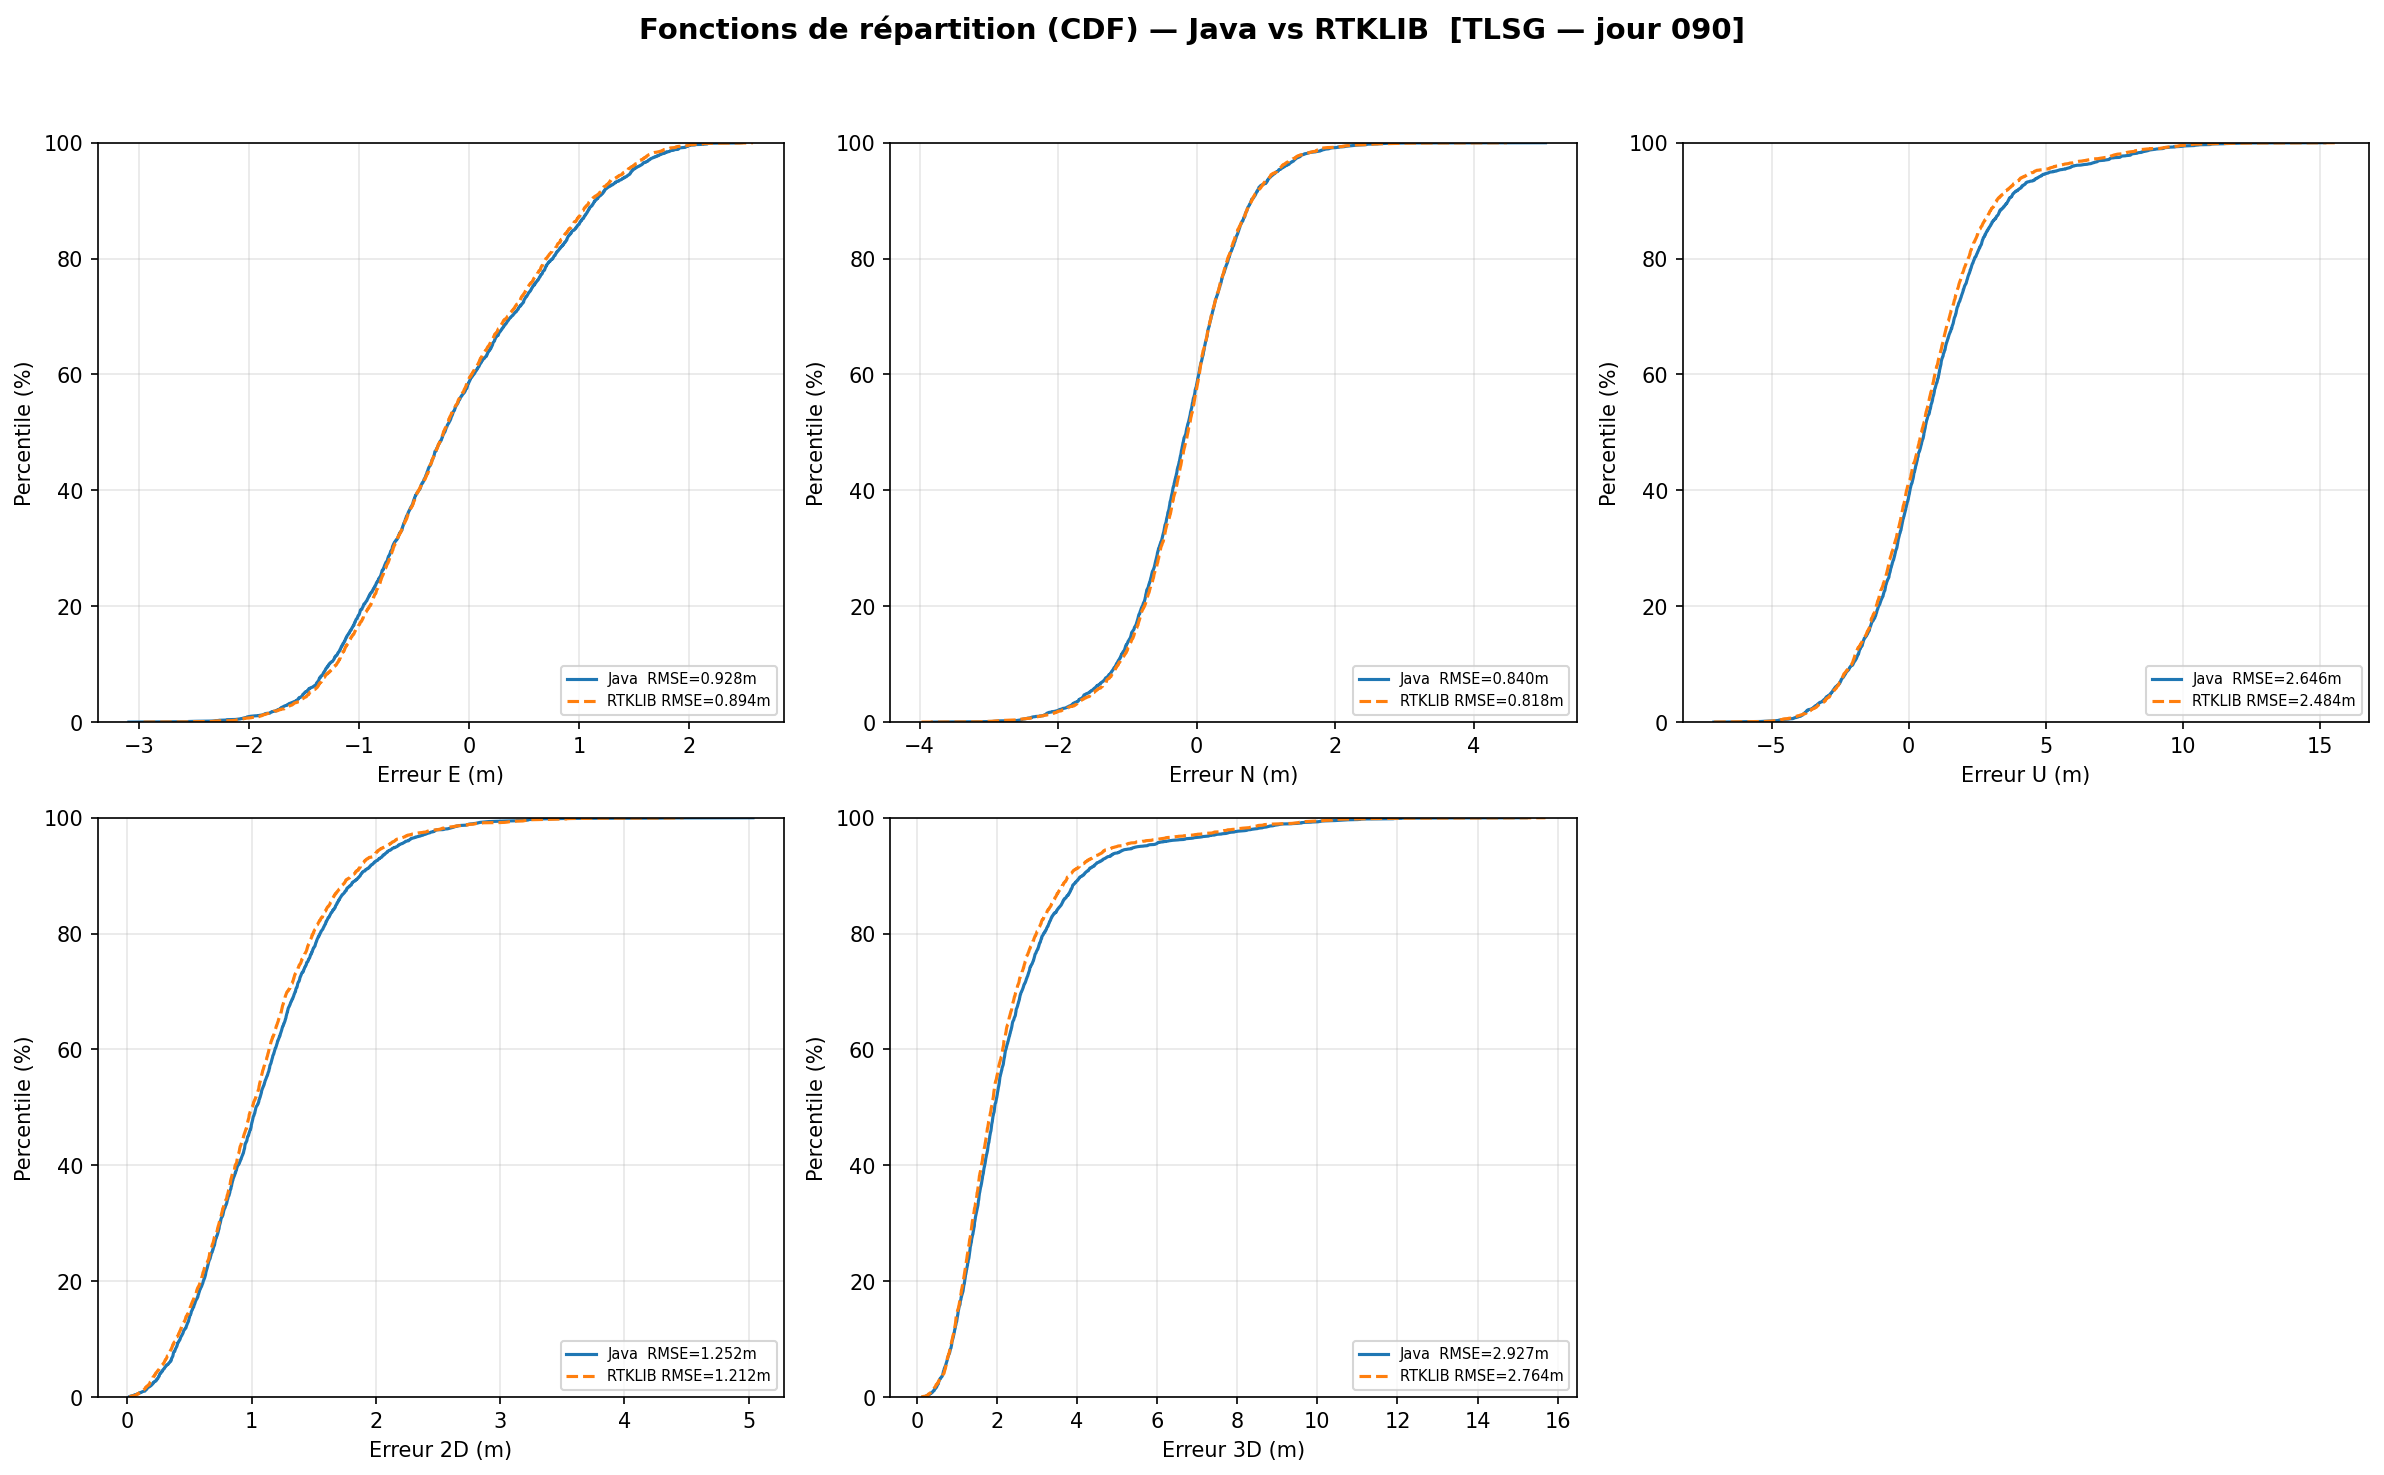
\includegraphics[width=\linewidth]{images/chapter5/ch5_wls_tlsg_j090_gps_if_saas_cdf.png}
    \end{minipage}
    \hspace{0.01\textwidth}
    \begin{minipage}[t]{0.64\textwidth}
        \centering
        \textbf{S-YEBE : YEBE}\par\medskip
        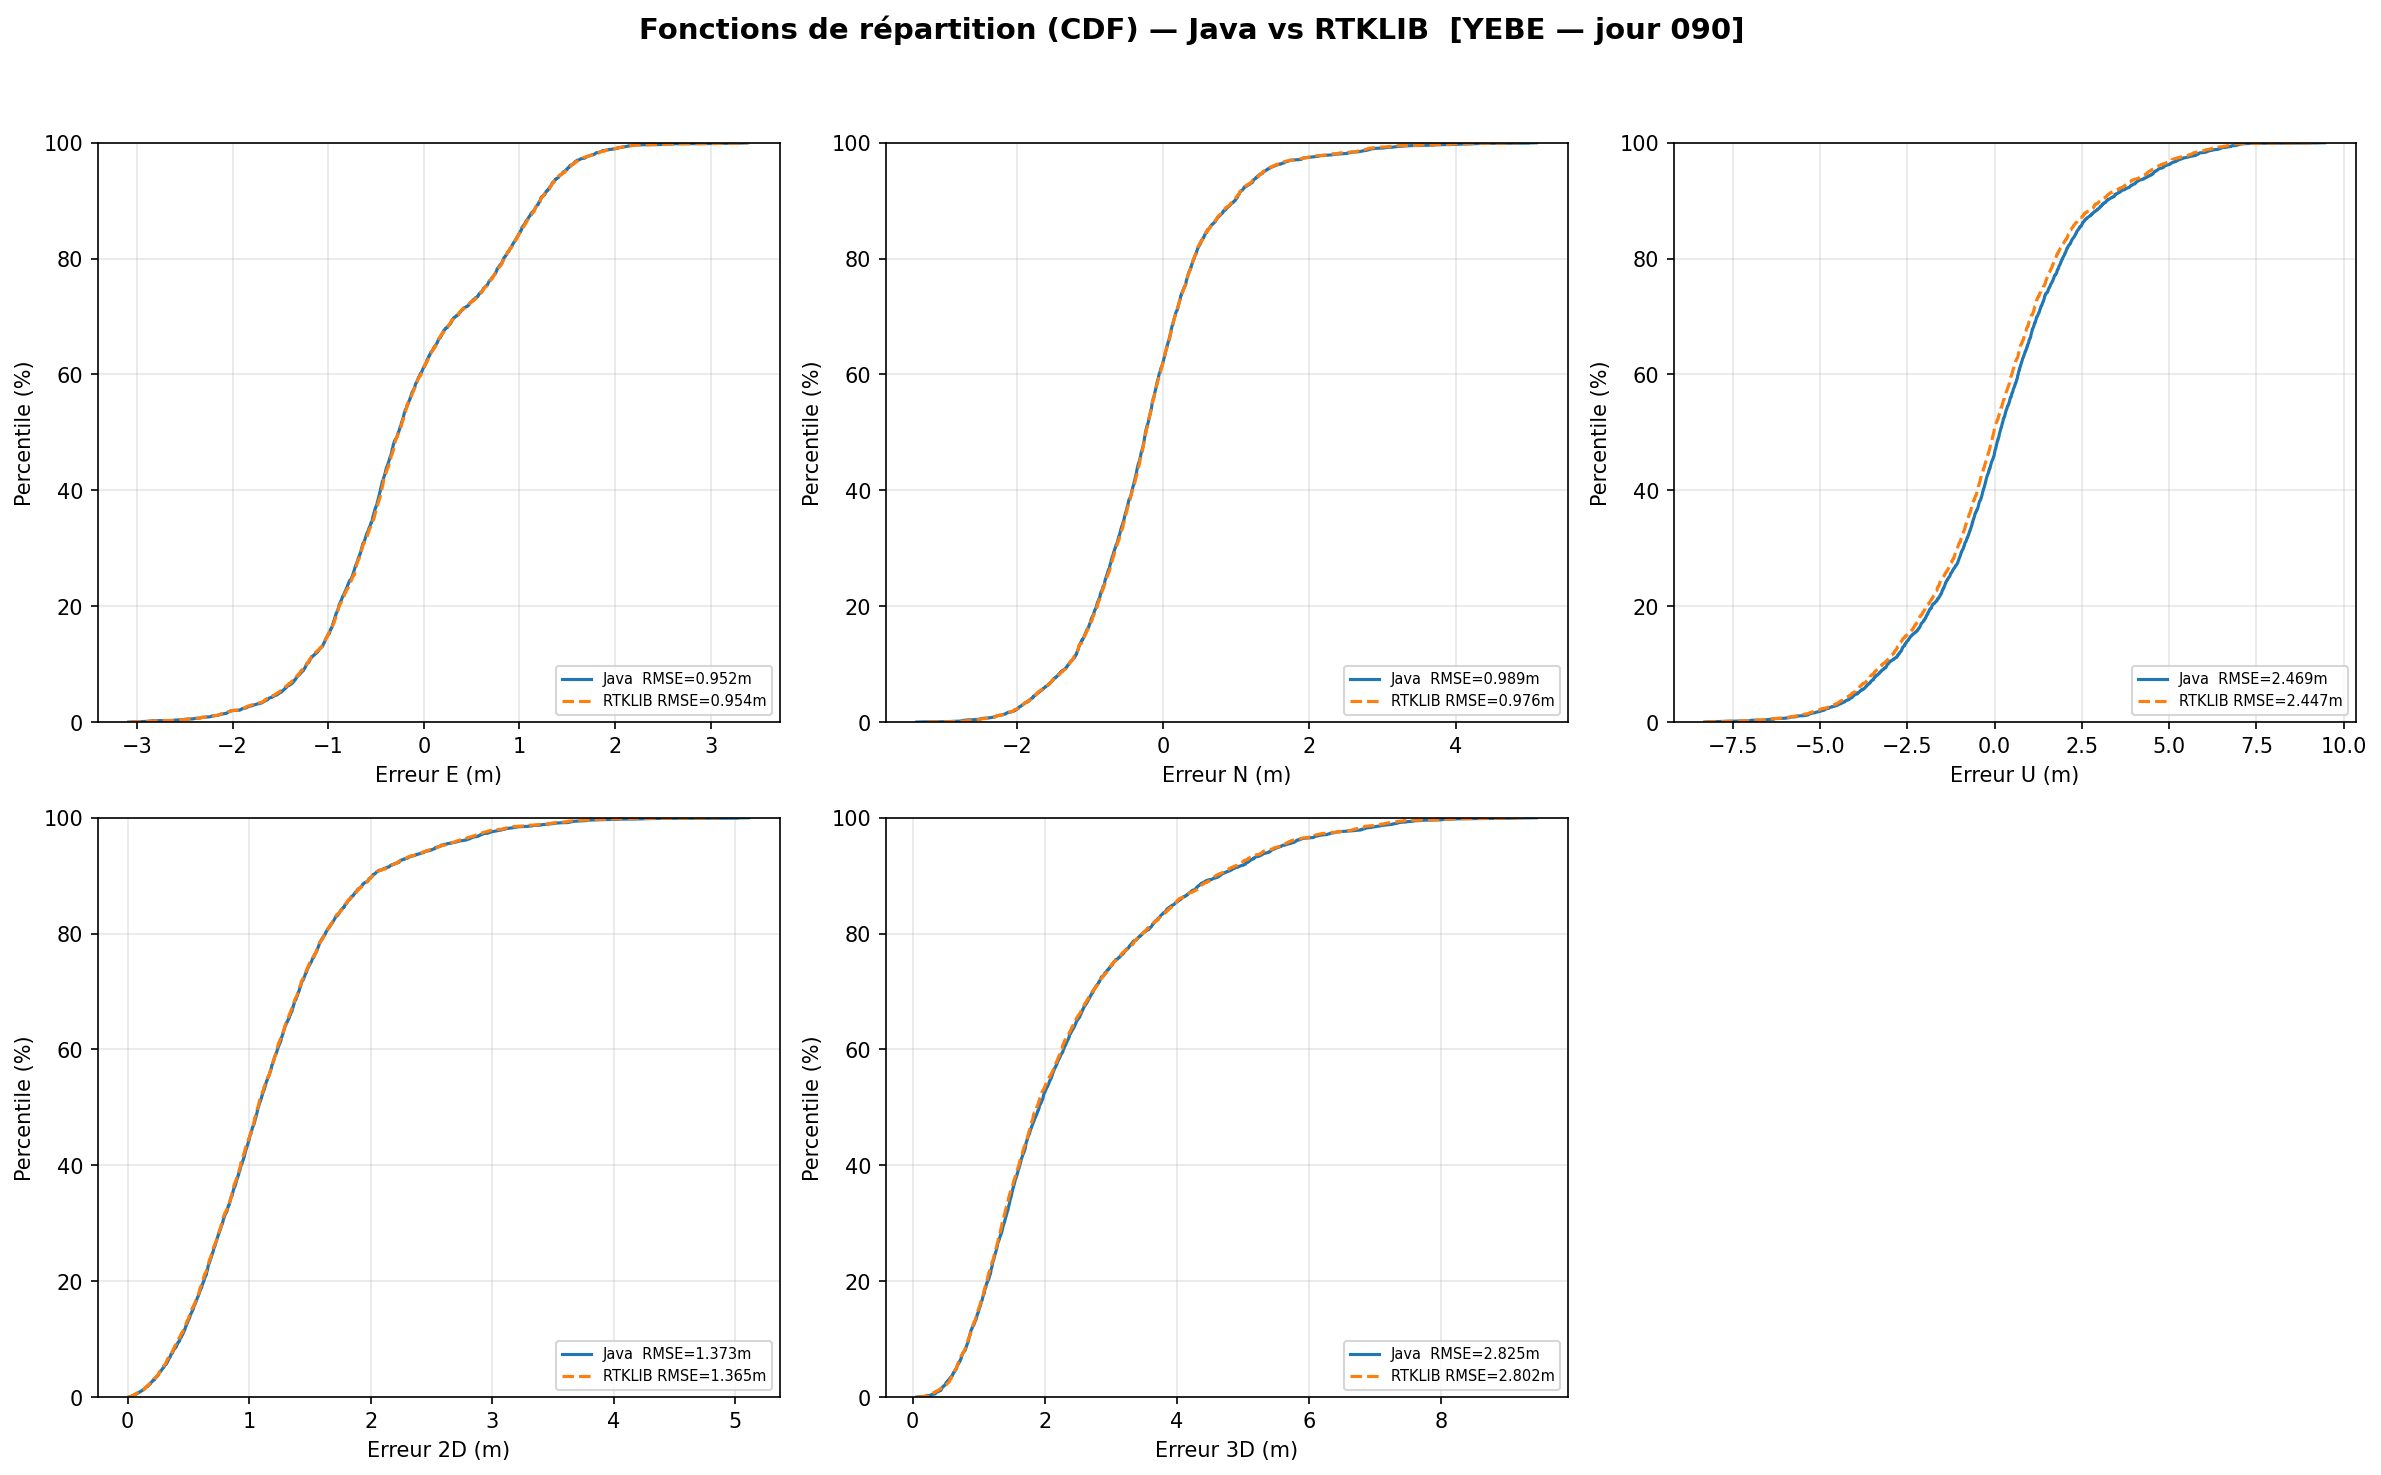
\includegraphics[width=\linewidth]{images/chapter5/ch5_wls_yebe_j090_gps_if_saas_cdf.png}
    \end{minipage}}
    \caption{Fonctions de répartition des erreurs pour le changement de
    station en mode Single.}
    \label{fig:ch5_single_station_cdf}
\end{figure}

Le changement de station modifie la géométrie satellite--récepteur,
l'environnement proche de l'antenne et les conditions atmosphériques. Il est
donc normal que la forme des nuages diffère. La RMSE 2D Java--Orekit passe de
$1{,}252$~m à TLSG à $1{,}373$~m à YEBE, sans variation d'ordre de grandeur.
Pour chacune des deux stations, les points Java--Orekit et RTKLIB se recouvrent
sur l'ensemble du nuage. Le comportement propre à chaque station est ainsi
fidèlement reproduit. Les CDF confirment ce résultat sur l'ensemble de la
distribution : à chaque station, les courbes des deux logiciels restent
proches, même si les distributions diffèrent entre TLSG et YEBE.

La figure~\ref{fig:ch5_single_ref_enu} présente les erreurs ENU de S-REF au
cours de la journée. Les variations temporelles Java--Orekit et RTKLIB sont
très proches sur les trois composantes. 

\begin{figure}[H]
    \centering
    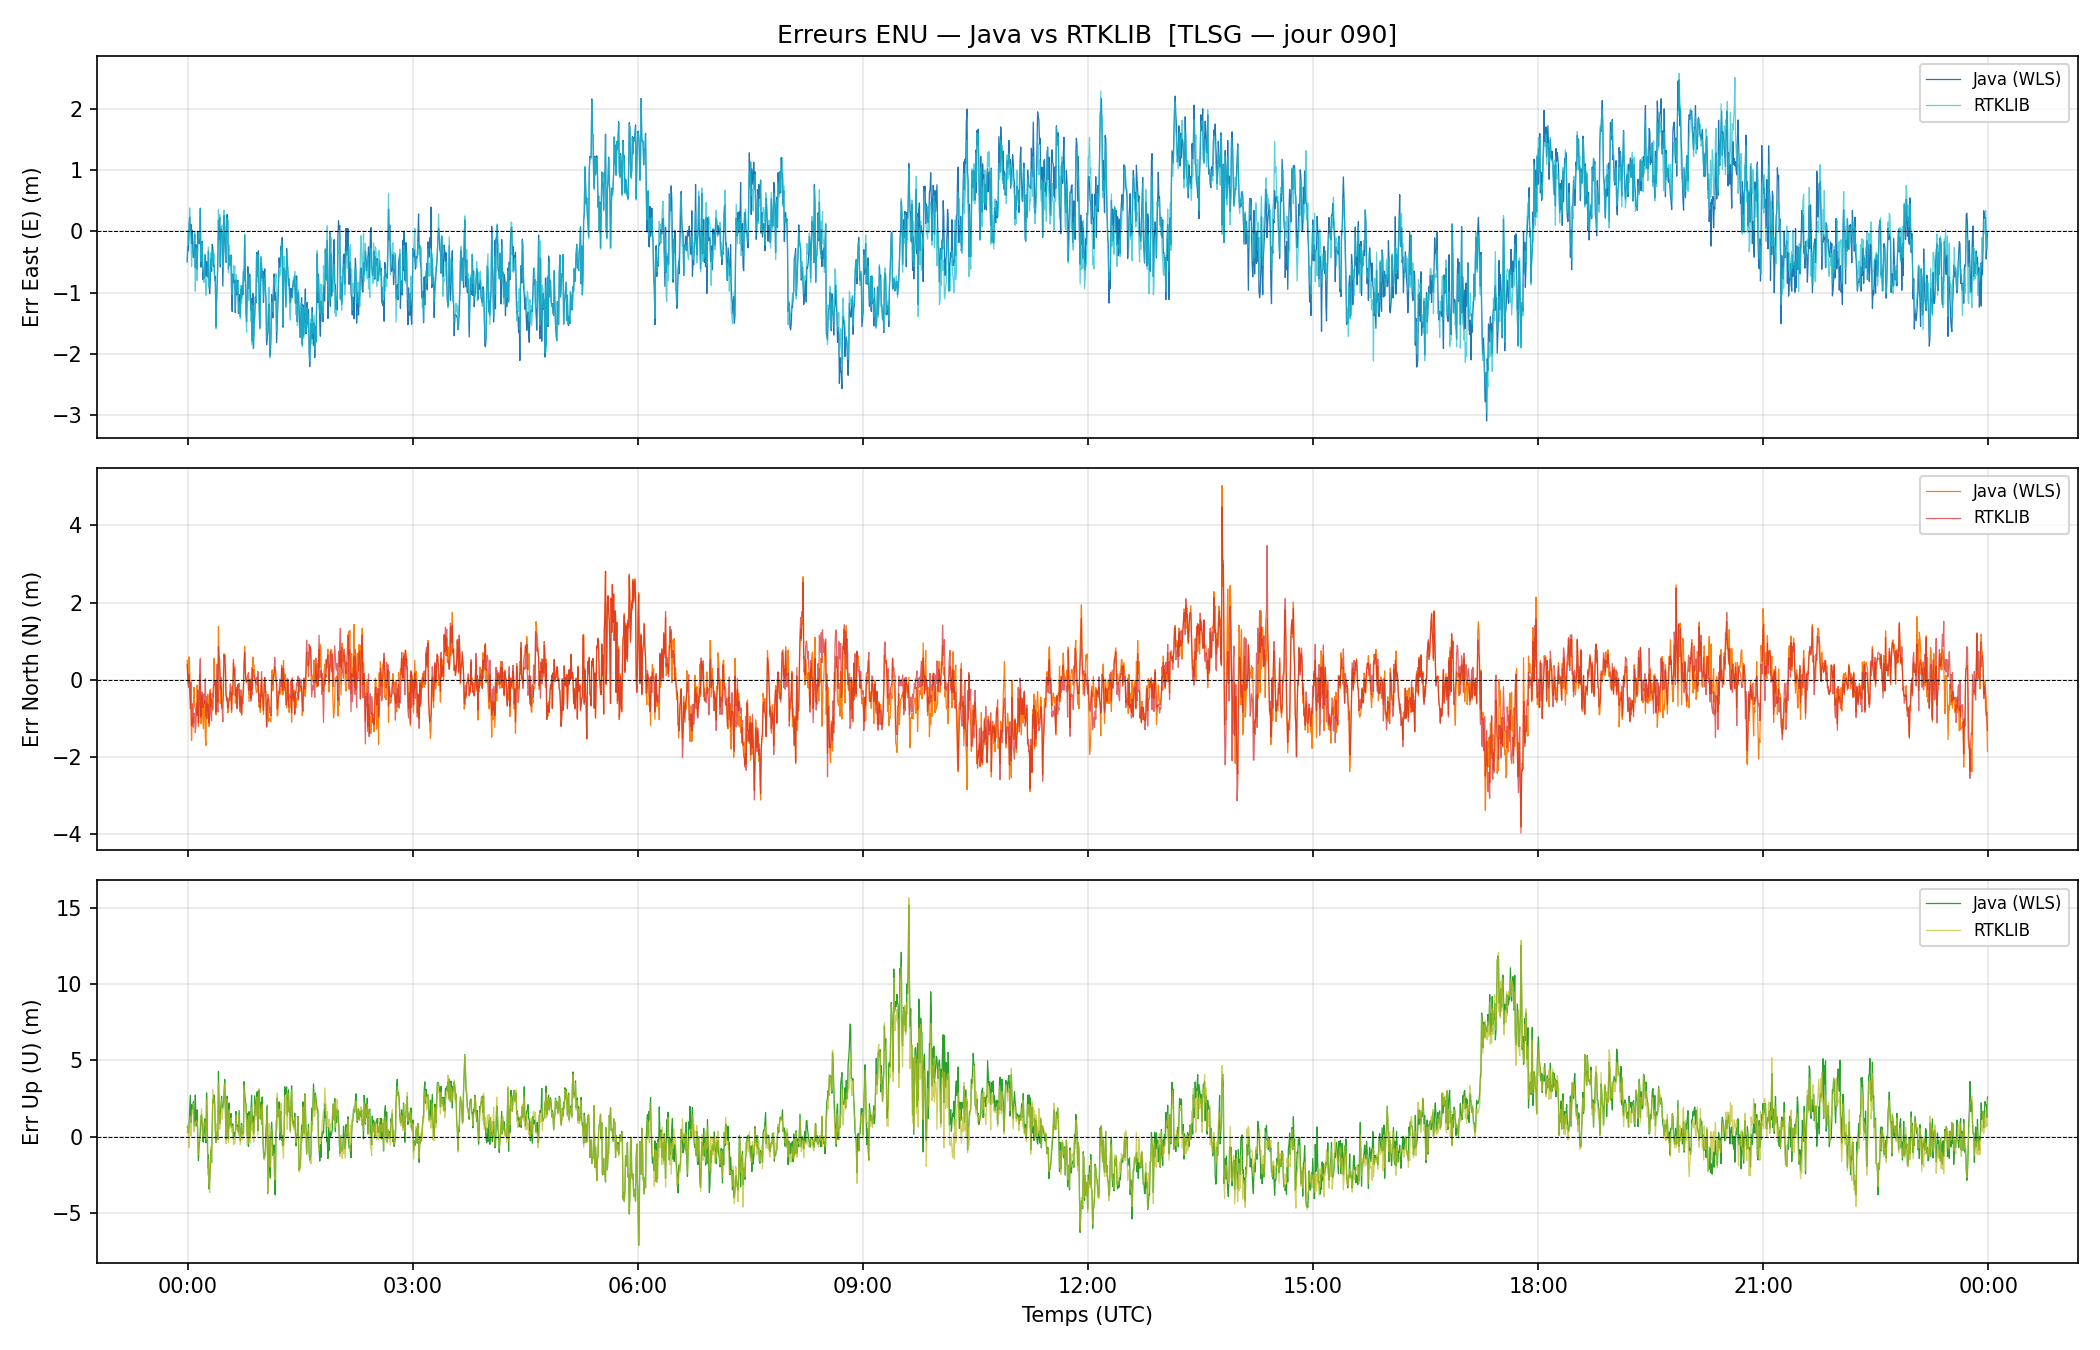
\includegraphics[width=\textwidth]{images/chapter5/ch5_wls_tlsg_j090_gps_if_saas_enu.png}
    \caption{Évolution des erreurs ENU de la référence Single S-REF.}
    \label{fig:ch5_single_ref_enu}
\end{figure}


\subsection{Ajout de Galileo}

Les figures~\ref{fig:ch5_single_galileo} et
\ref{fig:ch5_single_galileo_cdf} comparent S-REF à S-GAL. Seule la sélection
des constellations change : les observations Galileo sont ajoutées aux
observations GPS.

\begin{figure}[H]
    \centering
    \begin{minipage}[t]{0.48\textwidth}
        \centering
        \textbf{Référence S-REF : GPS}\par\medskip
        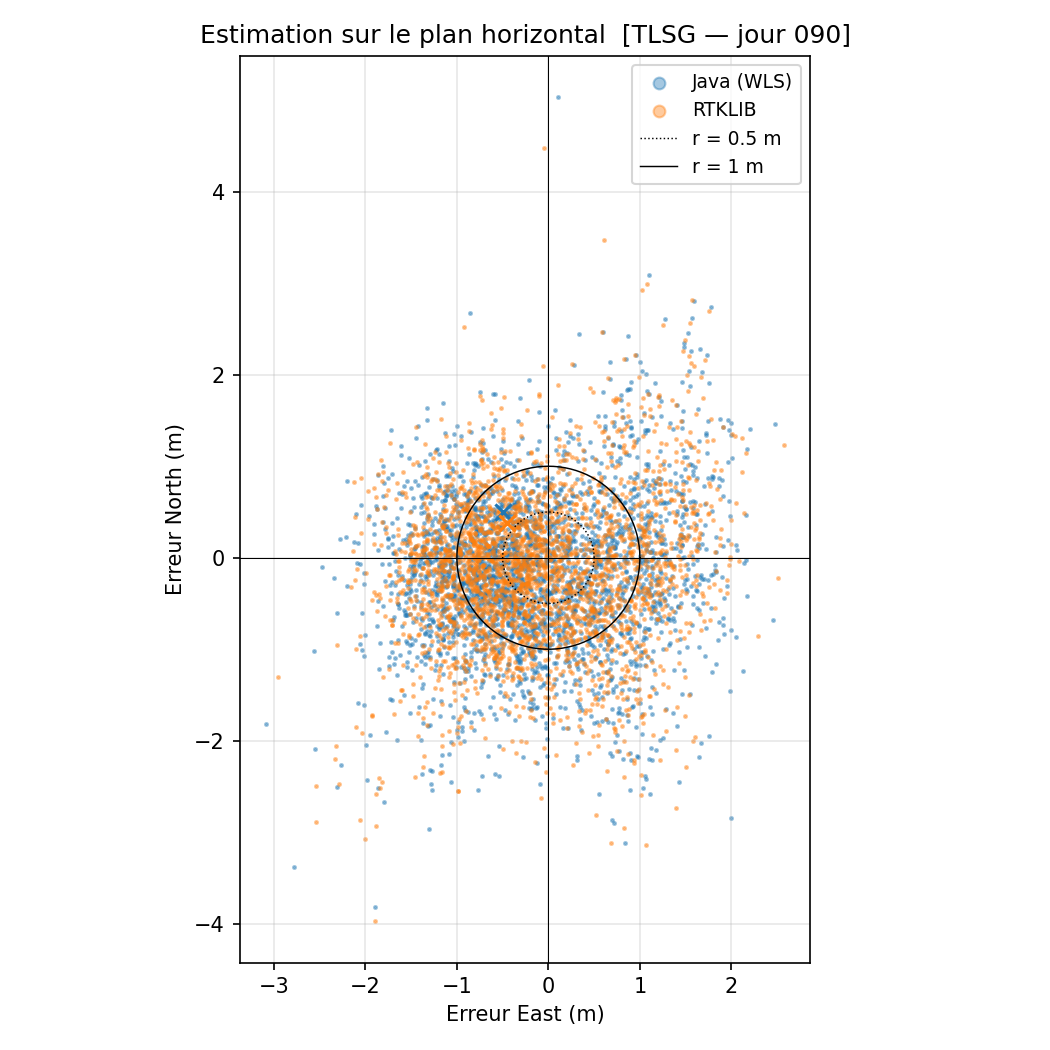
\includegraphics[width=\linewidth]{images/chapter5/ch5_wls_tlsg_j090_gps_if_saas_scatter_en.png}
    \end{minipage}
    \hfill
    \begin{minipage}[t]{0.48\textwidth}
        \centering
        \textbf{S-GAL : GPS+Galileo}\par\medskip
        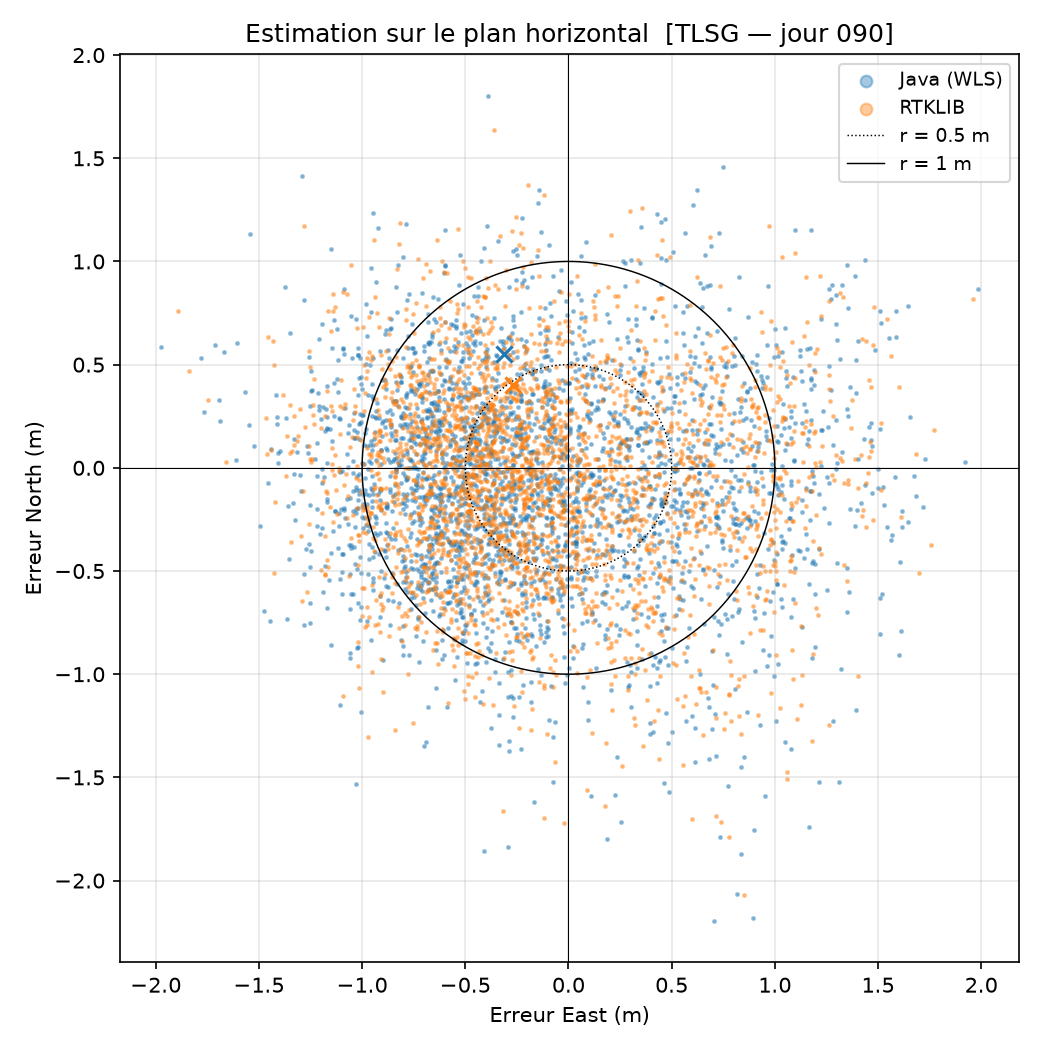
\includegraphics[width=\linewidth]{images/chapter5/ch5_wls_tlsg_j090_gpsgal_if_saas_scatter_en.png}
    \end{minipage}
    \caption{Effet de l'ajout de Galileo en mode Single à TLSG.}
    \label{fig:ch5_single_galileo}
\end{figure}

\begin{figure}[H]
    \centering
    \makebox[\textwidth][c]{%
    \begin{minipage}[t]{0.64\textwidth}
        \centering
        \textbf{Référence S-REF : GPS}\par\medskip
        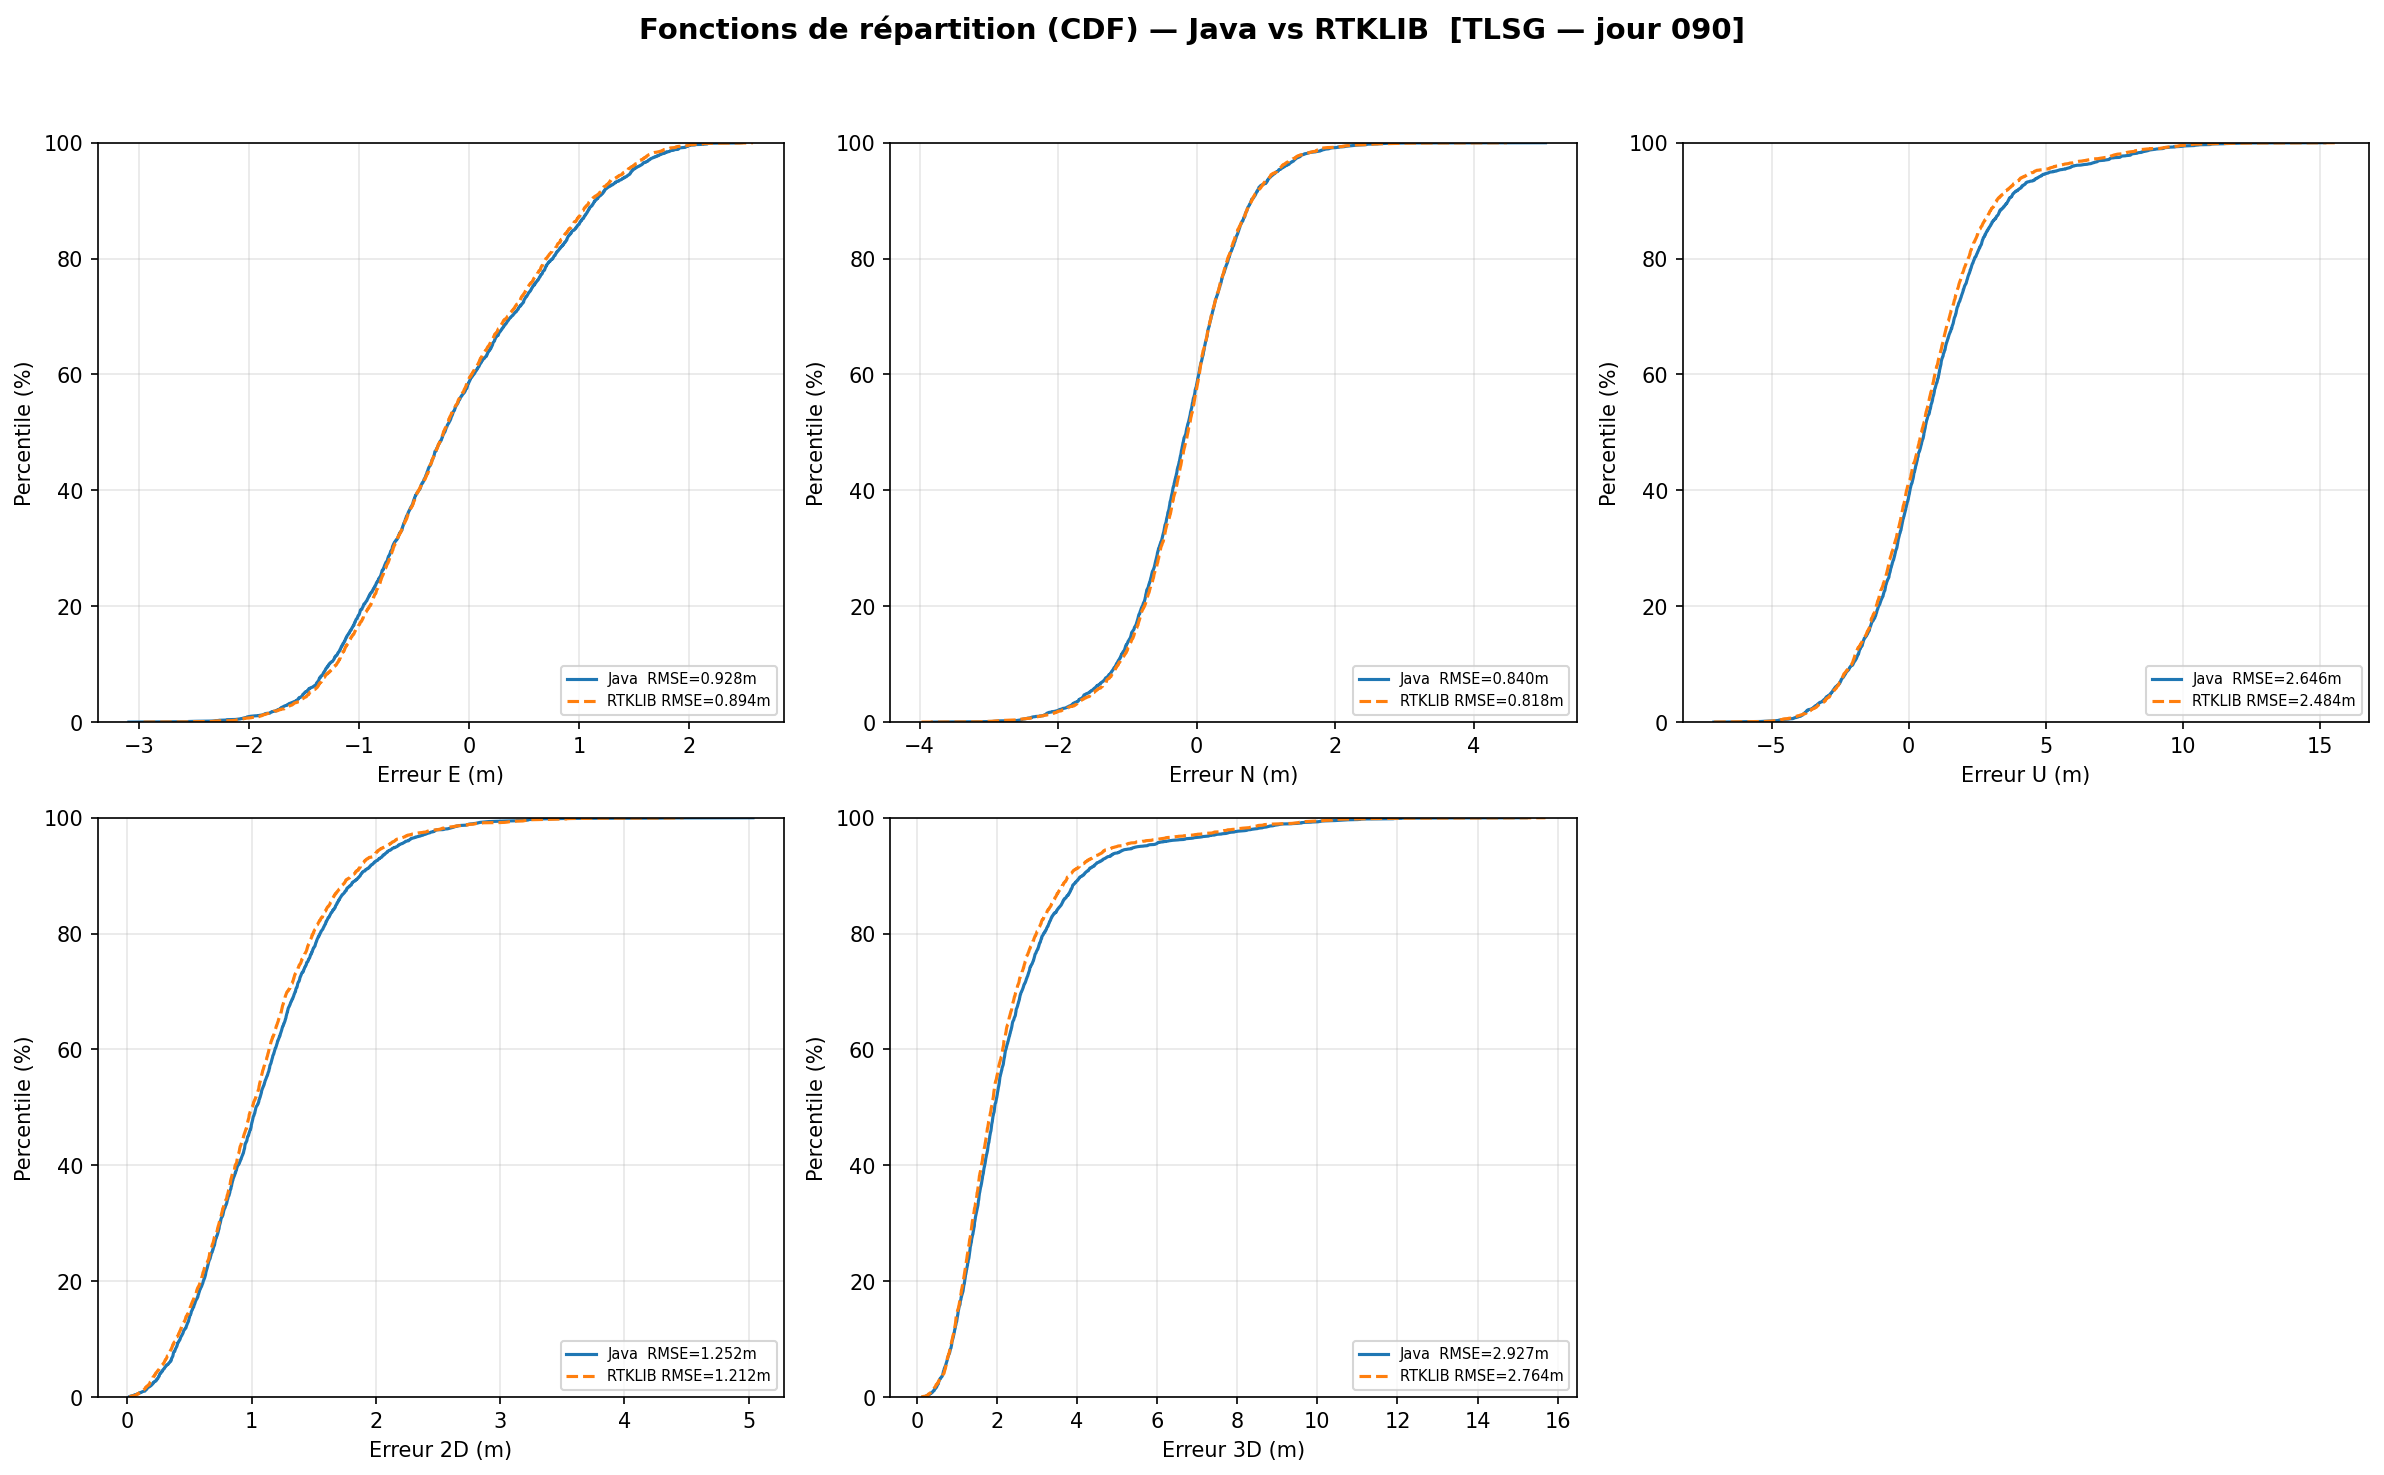
\includegraphics[width=\linewidth]{images/chapter5/ch5_wls_tlsg_j090_gps_if_saas_cdf.png}
    \end{minipage}
    \hspace{0.01\textwidth}
    \begin{minipage}[t]{0.64\textwidth}
        \centering
        \textbf{S-GAL : GPS+Galileo}\par\medskip
        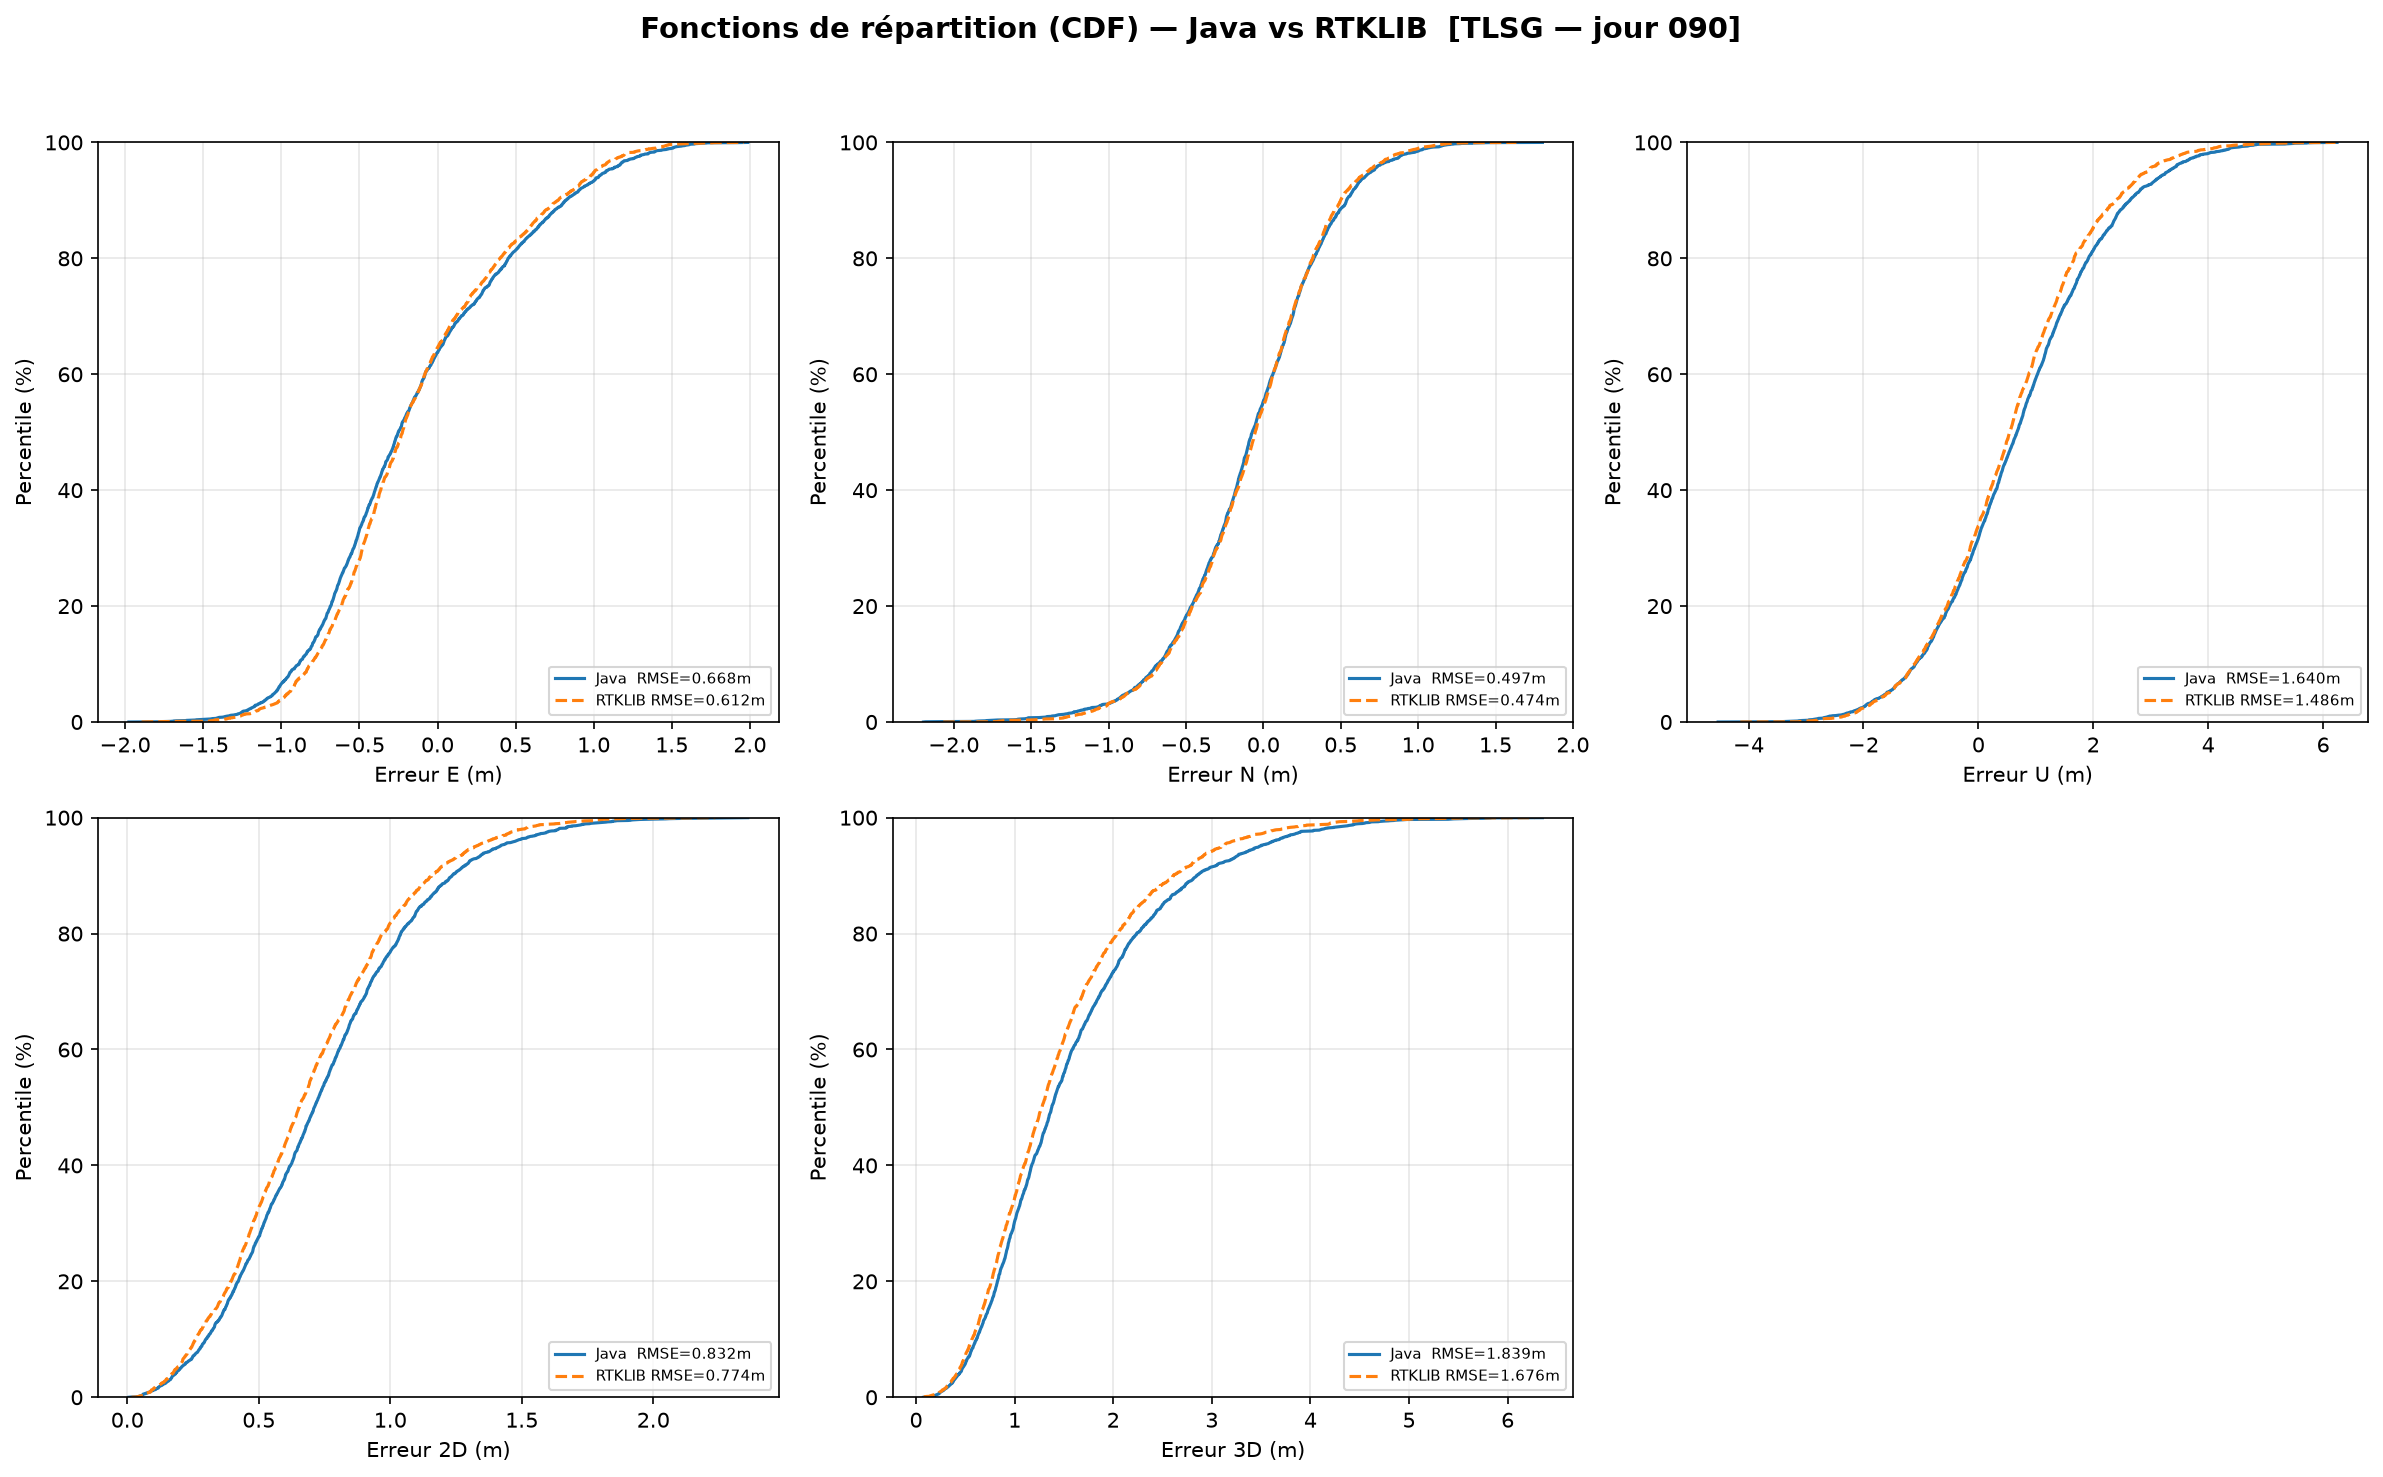
\includegraphics[width=\linewidth]{images/chapter5/ch5_wls_tlsg_j090_gpsgal_if_saas_cdf.png}
    \end{minipage}}
    \caption{Fonctions de répartition des erreurs avant et après l'ajout de
    Galileo.}
    \label{fig:ch5_single_galileo_cdf}
\end{figure}

L'ajout de Galileo augmente le nombre de satellites disponibles et diversifie
les directions d'observation. La matrice géométrique est alors mieux
conditionnée et le GDOP est réduit. Cet apport se traduit ici par
un nuage plus compact : la RMSE 2D Java--Orekit diminue de $1{,}252$ à
$0{,}832$~m. Le même resserrement apparaît dans RTKLIB, de $1{,}212$ à
$0{,}774$~m. Java--Orekit reste légèrement plus dispersé que RTKLIB dans le cas
GPS+Galileo, avec un écart de RMSE 2D de $5{,}8$~cm. Les deux nuages conservent
néanmoins la même forme et le même resserrement : l'amélioration apportée par
la multi-constellation est donc fidèlement reproduite. Le déplacement des CDF
2D et 3D vers les faibles erreurs confirme que le gain concerne l'ensemble de
la distribution et pas uniquement sa moyenne quadratique.


\subsection{Remplacement de la combinaison IF par Klobuchar}

Les figures~\ref{fig:ch5_single_klobuchar} et
\ref{fig:ch5_single_klobuchar_cdf} conservent la station, la constellation et
le modèle troposphérique de S-REF. Seule la correction ionosphérique est
remplacée par le modèle de Klobuchar.

\begin{figure}[H]
    \centering
    \begin{minipage}[t]{0.48\textwidth}
        \centering
        \textbf{Référence S-REF : IF}\par\medskip
        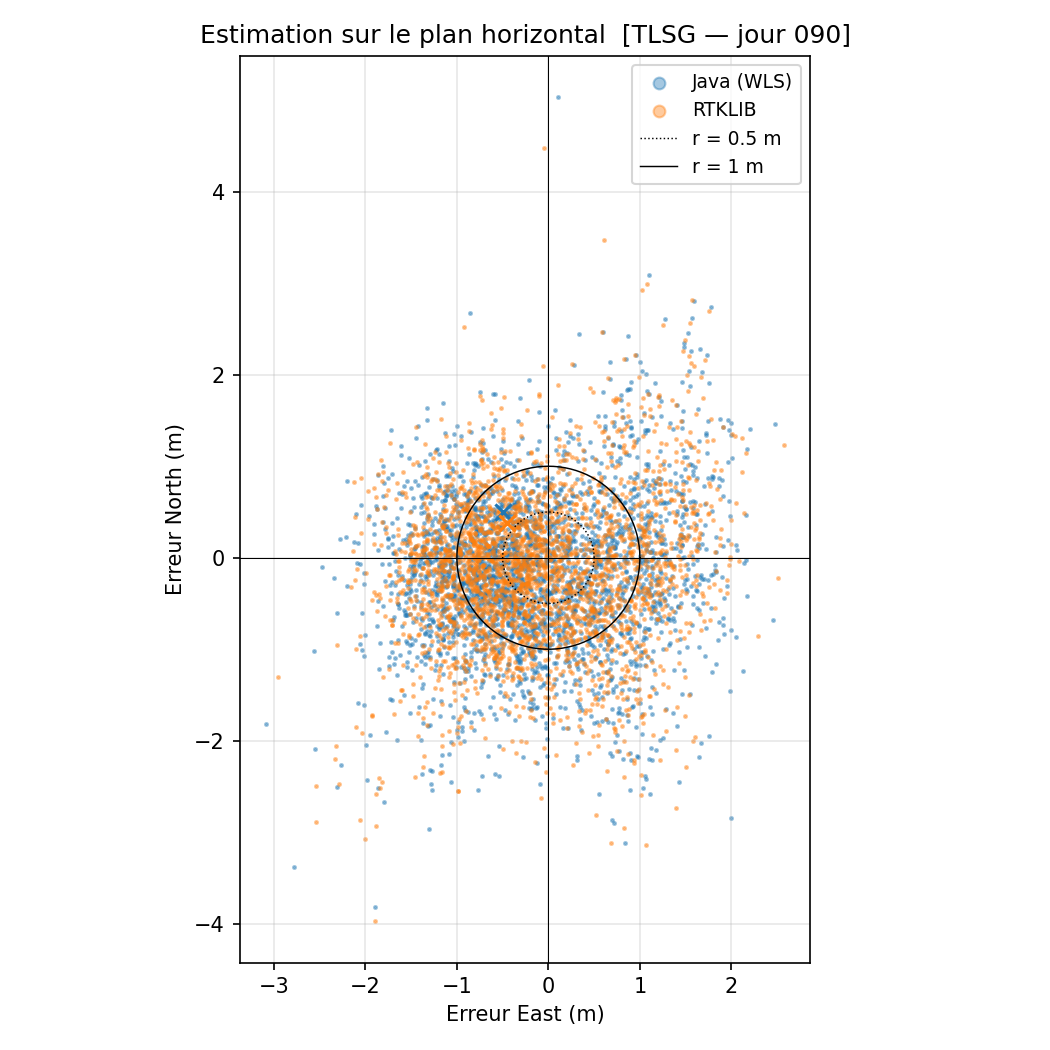
\includegraphics[width=\linewidth]{images/chapter5/ch5_wls_tlsg_j090_gps_if_saas_scatter_en.png}
    \end{minipage}
    \hfill
    \begin{minipage}[t]{0.48\textwidth}
        \centering
        \textbf{S-KLO : Klobuchar}\par\medskip
        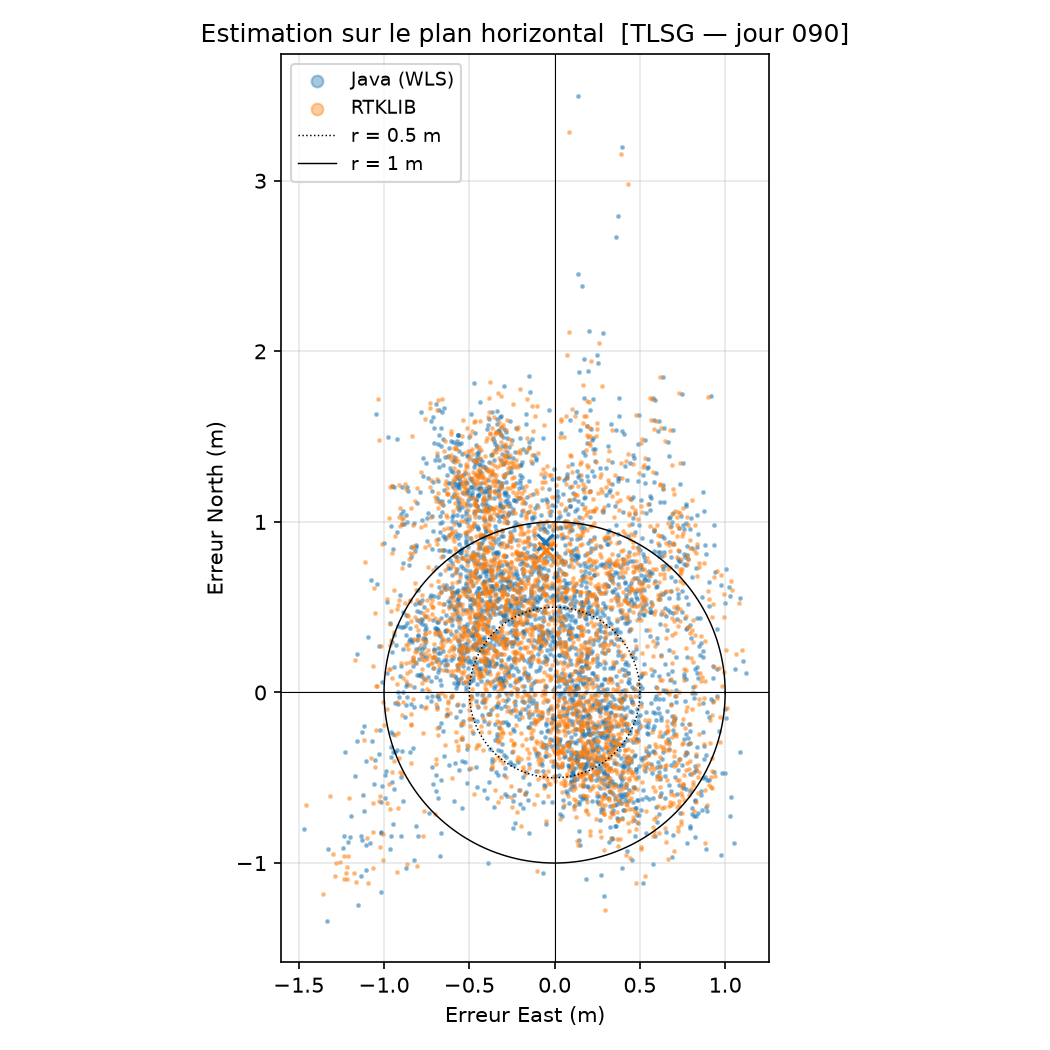
\includegraphics[width=\linewidth]{images/chapter5/ch5_wls_tlsg_j090_gps_klo_saas_scatter_en.png}
    \end{minipage}
    \caption{Effet du modèle ionosphérique en mode Single à TLSG.}
    \label{fig:ch5_single_klobuchar}
\end{figure}

\begin{figure}[H]
    \centering
    \makebox[\textwidth][c]{%
    \begin{minipage}[t]{0.64\textwidth}
        \centering
        \textbf{Référence S-REF : IF}\par\medskip
        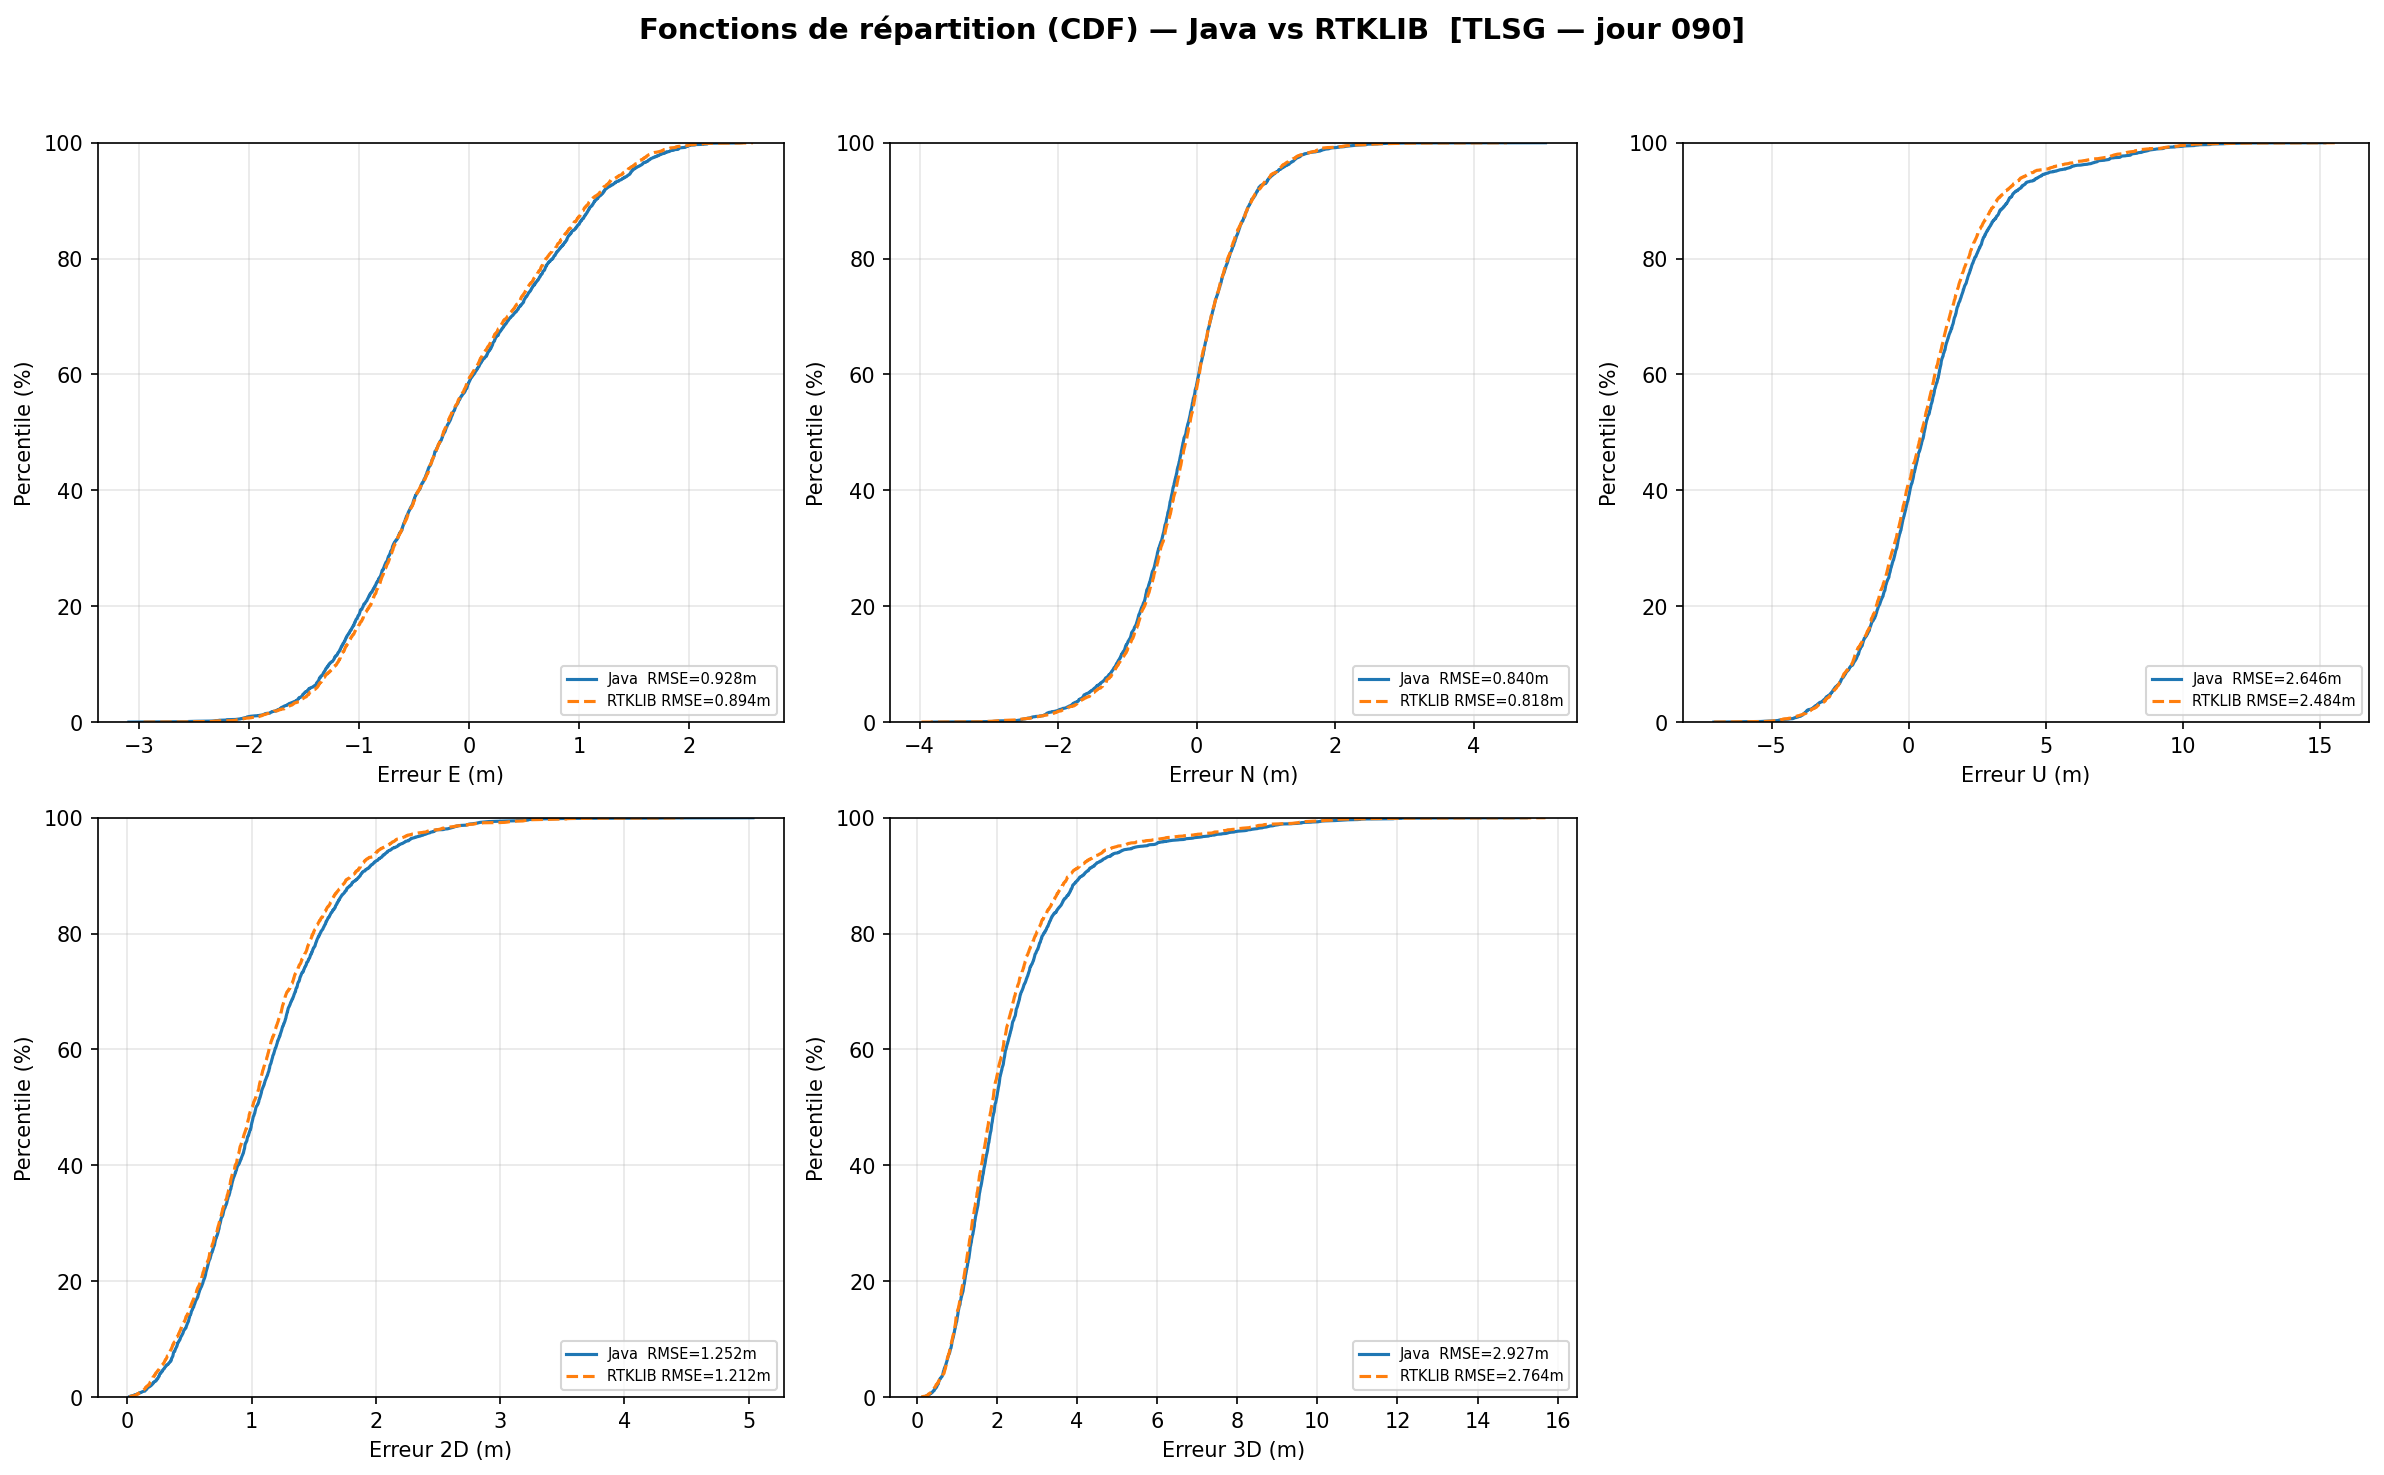
\includegraphics[width=\linewidth]{images/chapter5/ch5_wls_tlsg_j090_gps_if_saas_cdf.png}
    \end{minipage}
    \hspace{0.01\textwidth}
    \begin{minipage}[t]{0.64\textwidth}
        \centering
        \textbf{S-KLO : Klobuchar}\par\medskip
        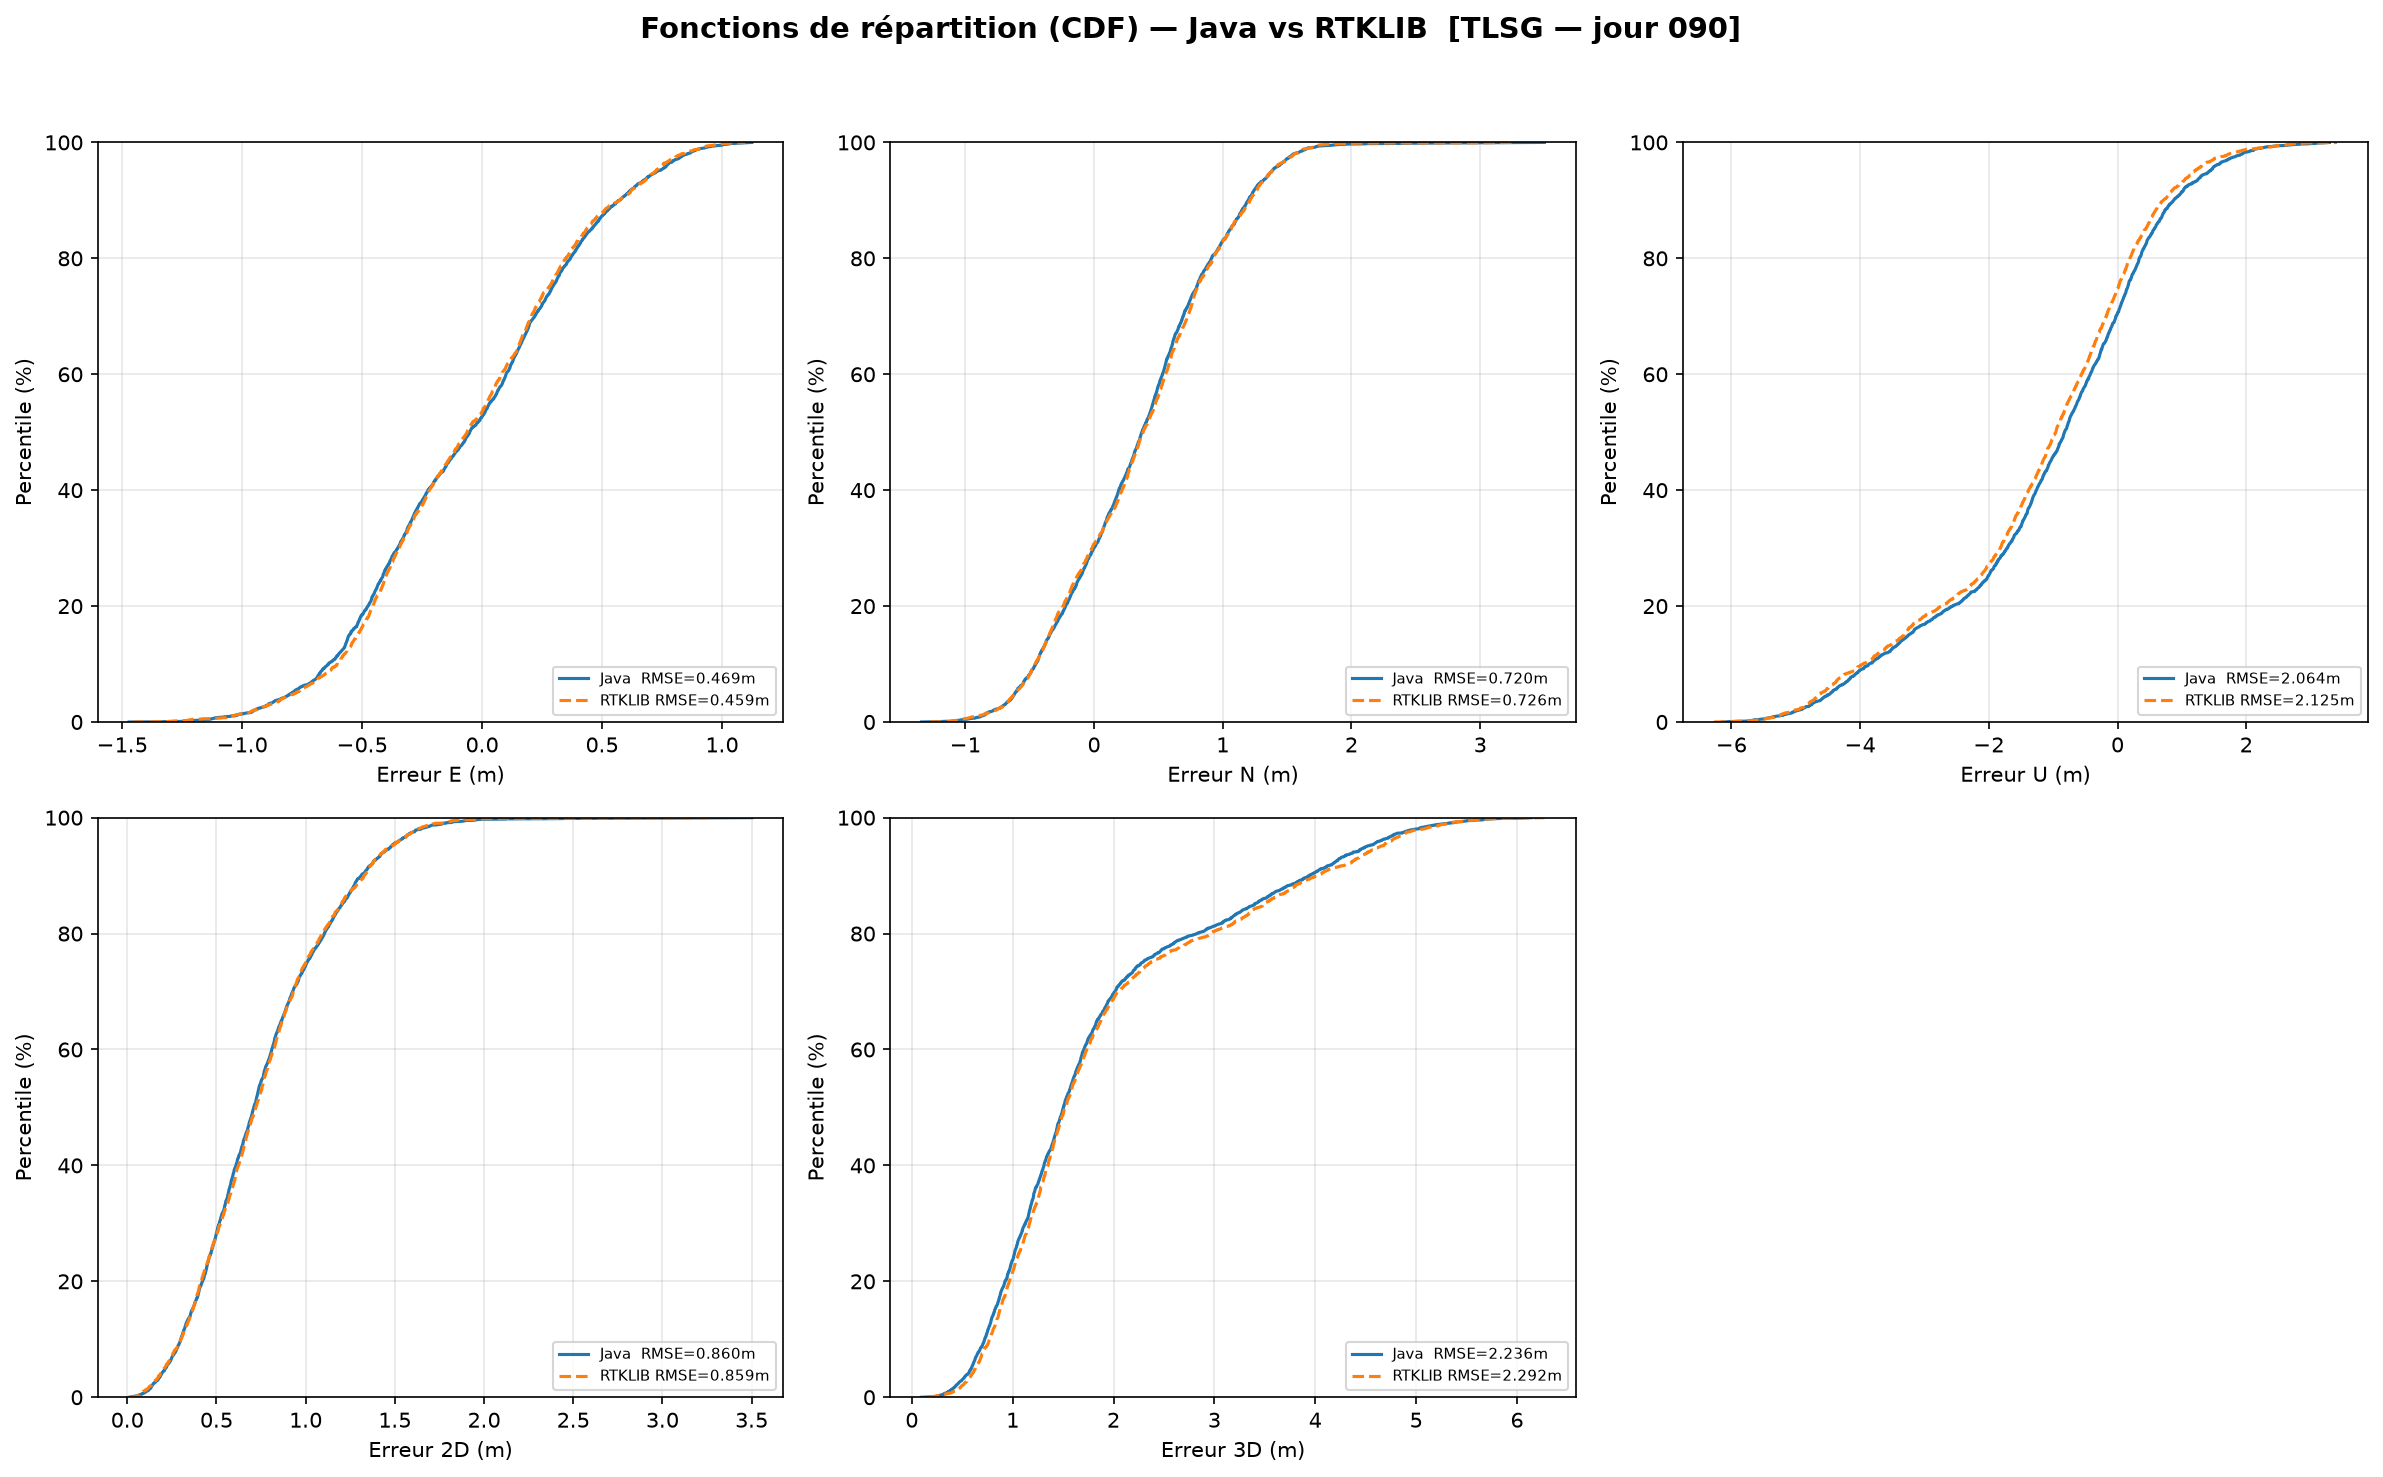
\includegraphics[width=\linewidth]{images/chapter5/ch5_wls_tlsg_j090_gps_klo_saas_cdf.png}
    \end{minipage}}
    \caption{Fonctions de répartition des erreurs pour les deux traitements
    ionosphériques.}
    \label{fig:ch5_single_klobuchar_cdf}
\end{figure}

La combinaison iono-free élimine le terme ionosphérique du premier
ordre, mais amplifie le bruit des mesures de code lors de la combinaison des
deux fréquences. Klobuchar ne supprime qu'une partie du retard ionosphérique,
mais conserve le niveau de bruit d'une observation mono-fréquence. Sur cette
journée, ce compromis conduit à une dispersion horizontale plus faible avec
Klobuchar : la RMSE 2D Java--Orekit passe de $1{,}252$ à $0{,}860$~m. RTKLIB
présente la même évolution, de $1{,}212$ à $0{,}859$~m. Dans le cas KLO, les
RMSE 2D des deux logiciels ne diffèrent que d'un millimètre. Cette
conclusion est propre aux données étudiées et ne signifie pas que Klobuchar est
systématiquement plus exact. Les trajectoires Java--Orekit et RTKLIB restent
presque confondues dans les deux modes, ce qui valide les deux traitements
ionosphériques. Les CDF Java--Orekit et RTKLIB du cas KLO sont elles aussi
presque confondues, notamment pour les erreurs horizontales et 2D.


\section{Validation de l'EKF avec éphémérides diffusées}
\label{sec:validation_ekf_broadcast}

\subsection{Configuration EKF de référence et estimation de la troposphère}

E-REF constitue la référence EKF : code et phase, GPS, combinaison
iono-free, modèle SAAS et éphémérides diffusées. E-GRAD conserve tous
ces choix, mais remplace la correction troposphérique déterministe par
l'estimation du ZTD et de deux gradients horizontaux. Les nuages sont comparés
sur la figure~\ref{fig:ch5_ekf_tropo} et les erreurs ENU sur la
figure~\ref{fig:ch5_ekf_tropo_enu}.

\begin{figure}[H]
    \centering
    \begin{minipage}[t]{0.48\textwidth}
        \centering
        \textbf{Référence E-REF : SAAS}\par\medskip
        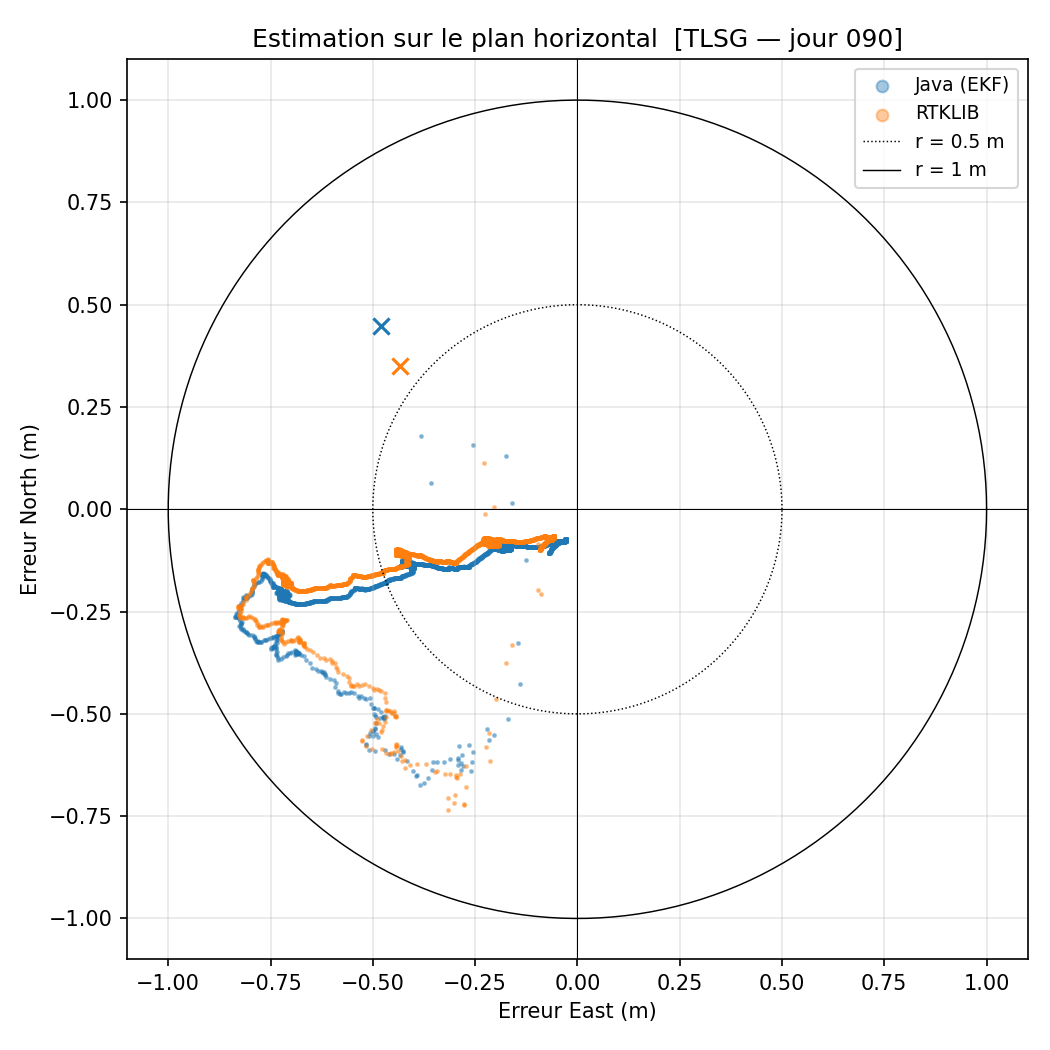
\includegraphics[width=\linewidth]{images/chapter5/ch5_ekf_tlsg_j090_gps_if_saas_scatter_en.png}
    \end{minipage}
    \hfill
    \begin{minipage}[t]{0.48\textwidth}
        \centering
        \textbf{E-GRAD : ZTD+GRAD}\par\medskip
        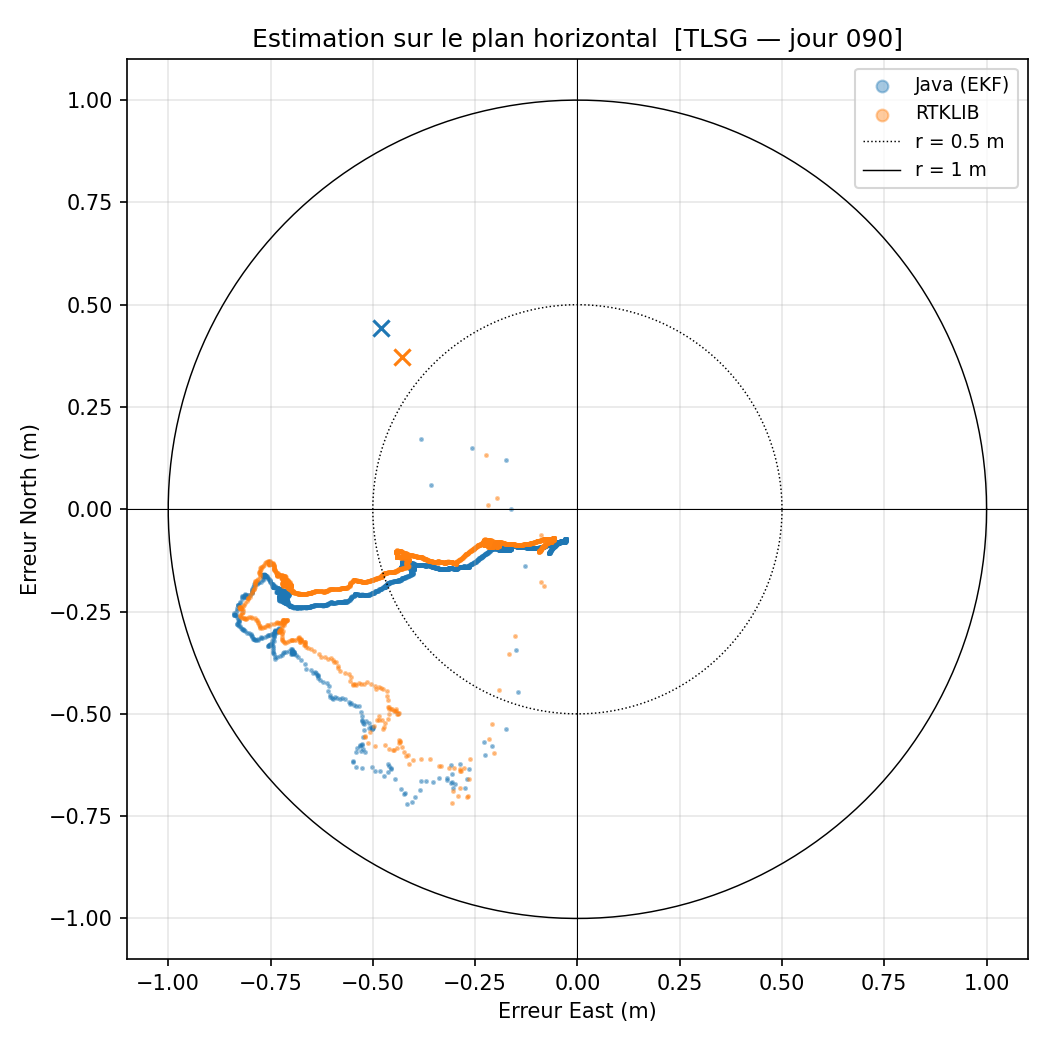
\includegraphics[width=\linewidth]{images/chapter5/ch5_ekf_tlsg_j090_gps_if_ztdgrad_broadcast_scatter_en.png}
    \end{minipage}
    \caption{Effet de l'estimation troposphérique dans l'EKF avec
    éphémérides diffusées.}
    \label{fig:ch5_ekf_tropo}
\end{figure}

\begin{figure}[H]
    \centering
    \makebox[\textwidth][c]{%
    \begin{minipage}[t]{0.64\textwidth}
        \centering
        \textbf{Référence E-REF : SAAS}\par\medskip
        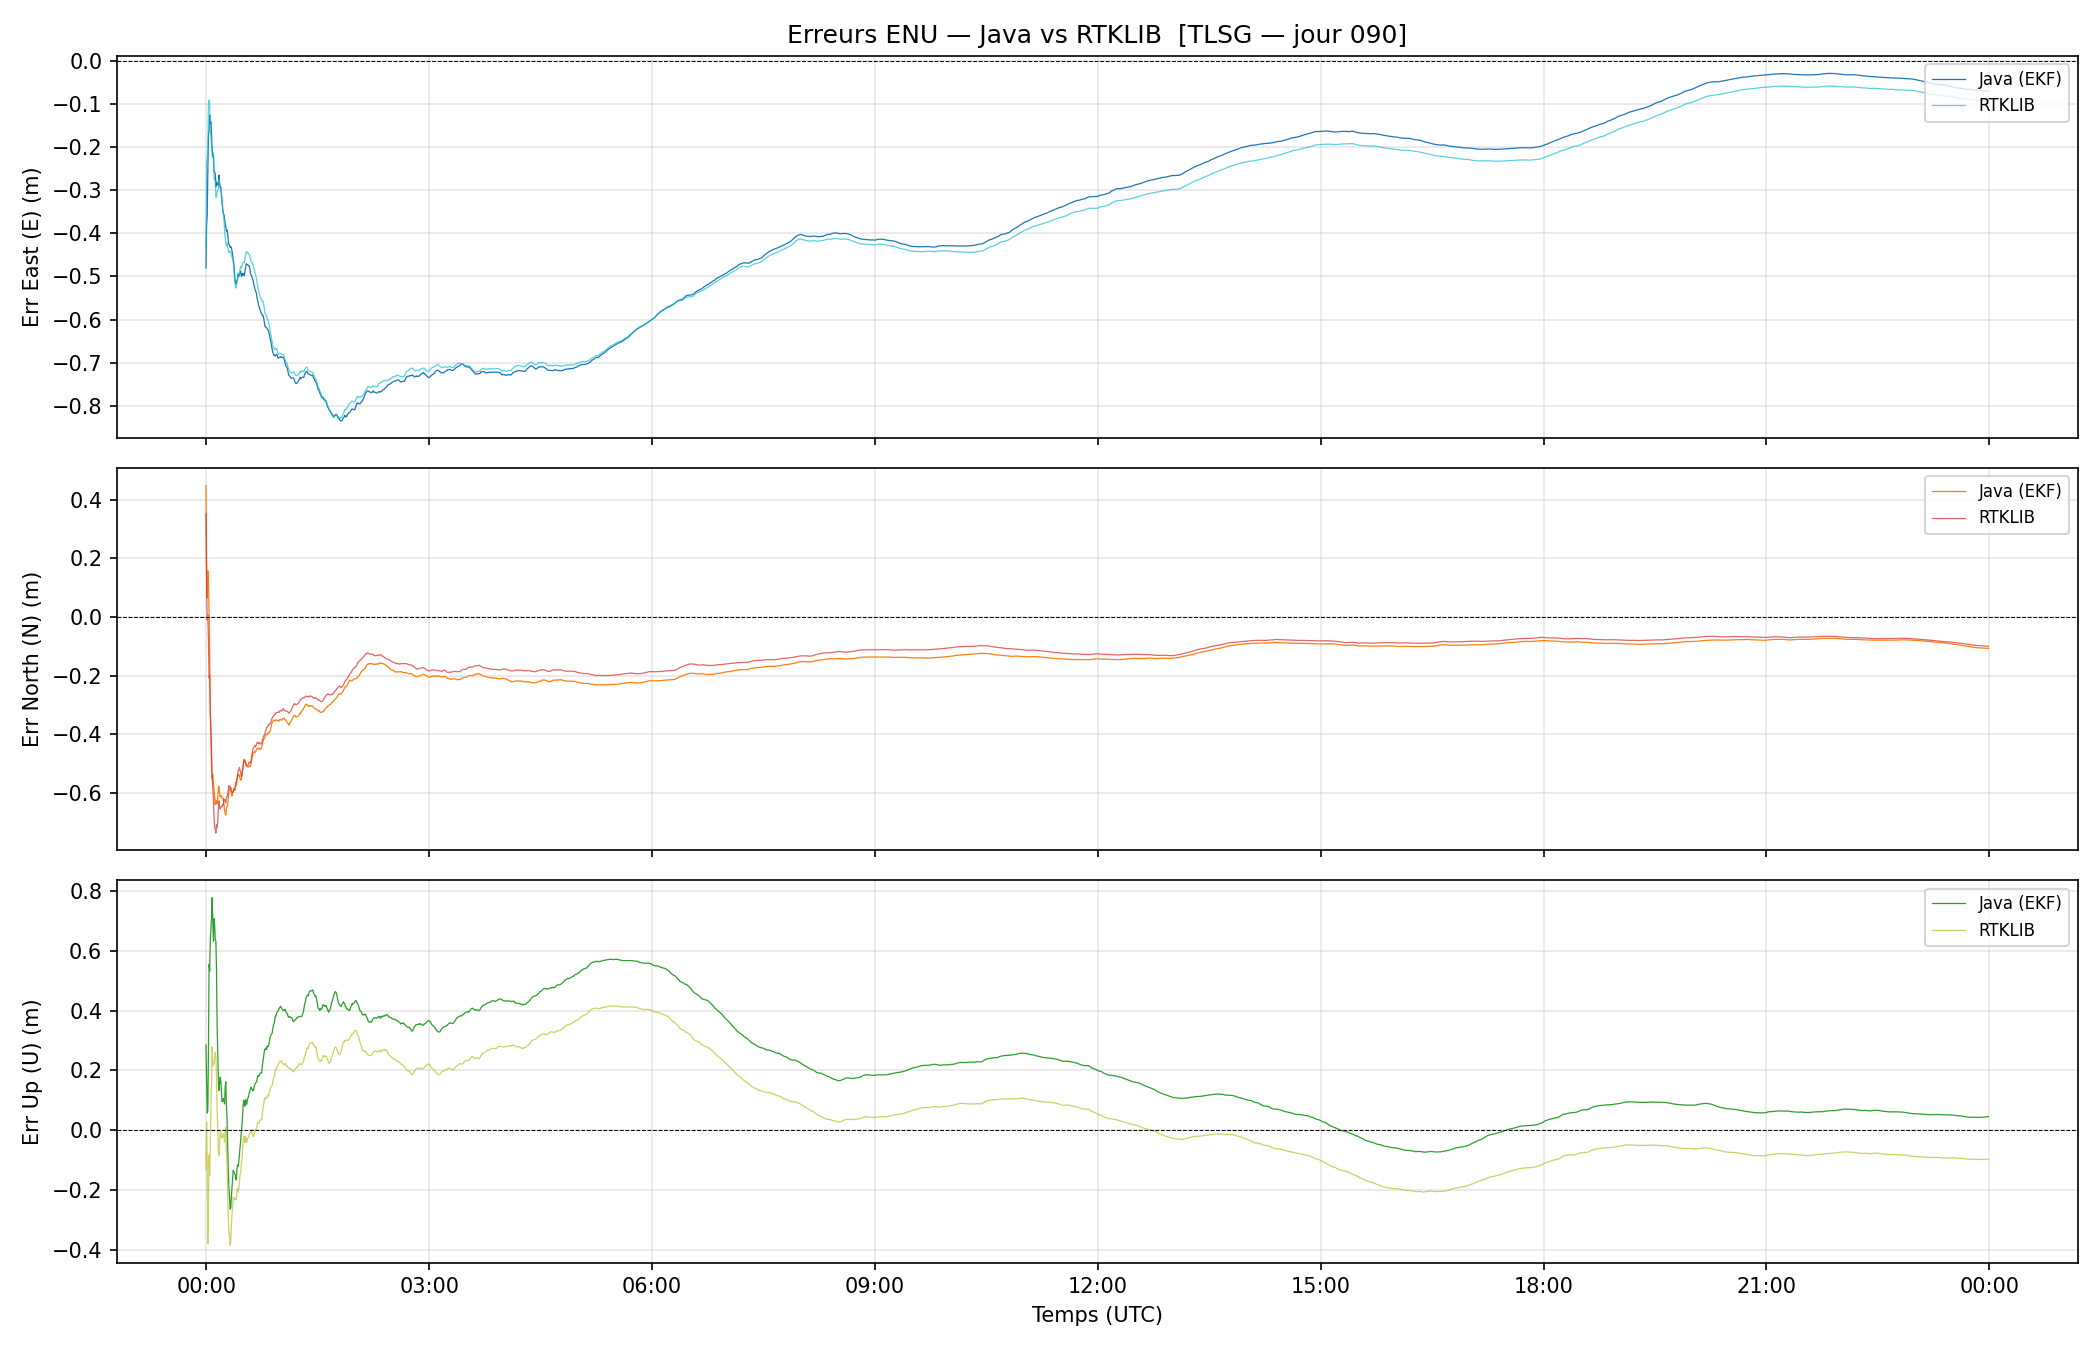
\includegraphics[width=\linewidth]{images/chapter5/ch5_ekf_tlsg_j090_gps_if_saas_enu.png}
    \end{minipage}
    \hspace{0.01\textwidth}
    \begin{minipage}[t]{0.64\textwidth}
        \centering
        \textbf{E-GRAD : ZTD+GRAD}\par\medskip
        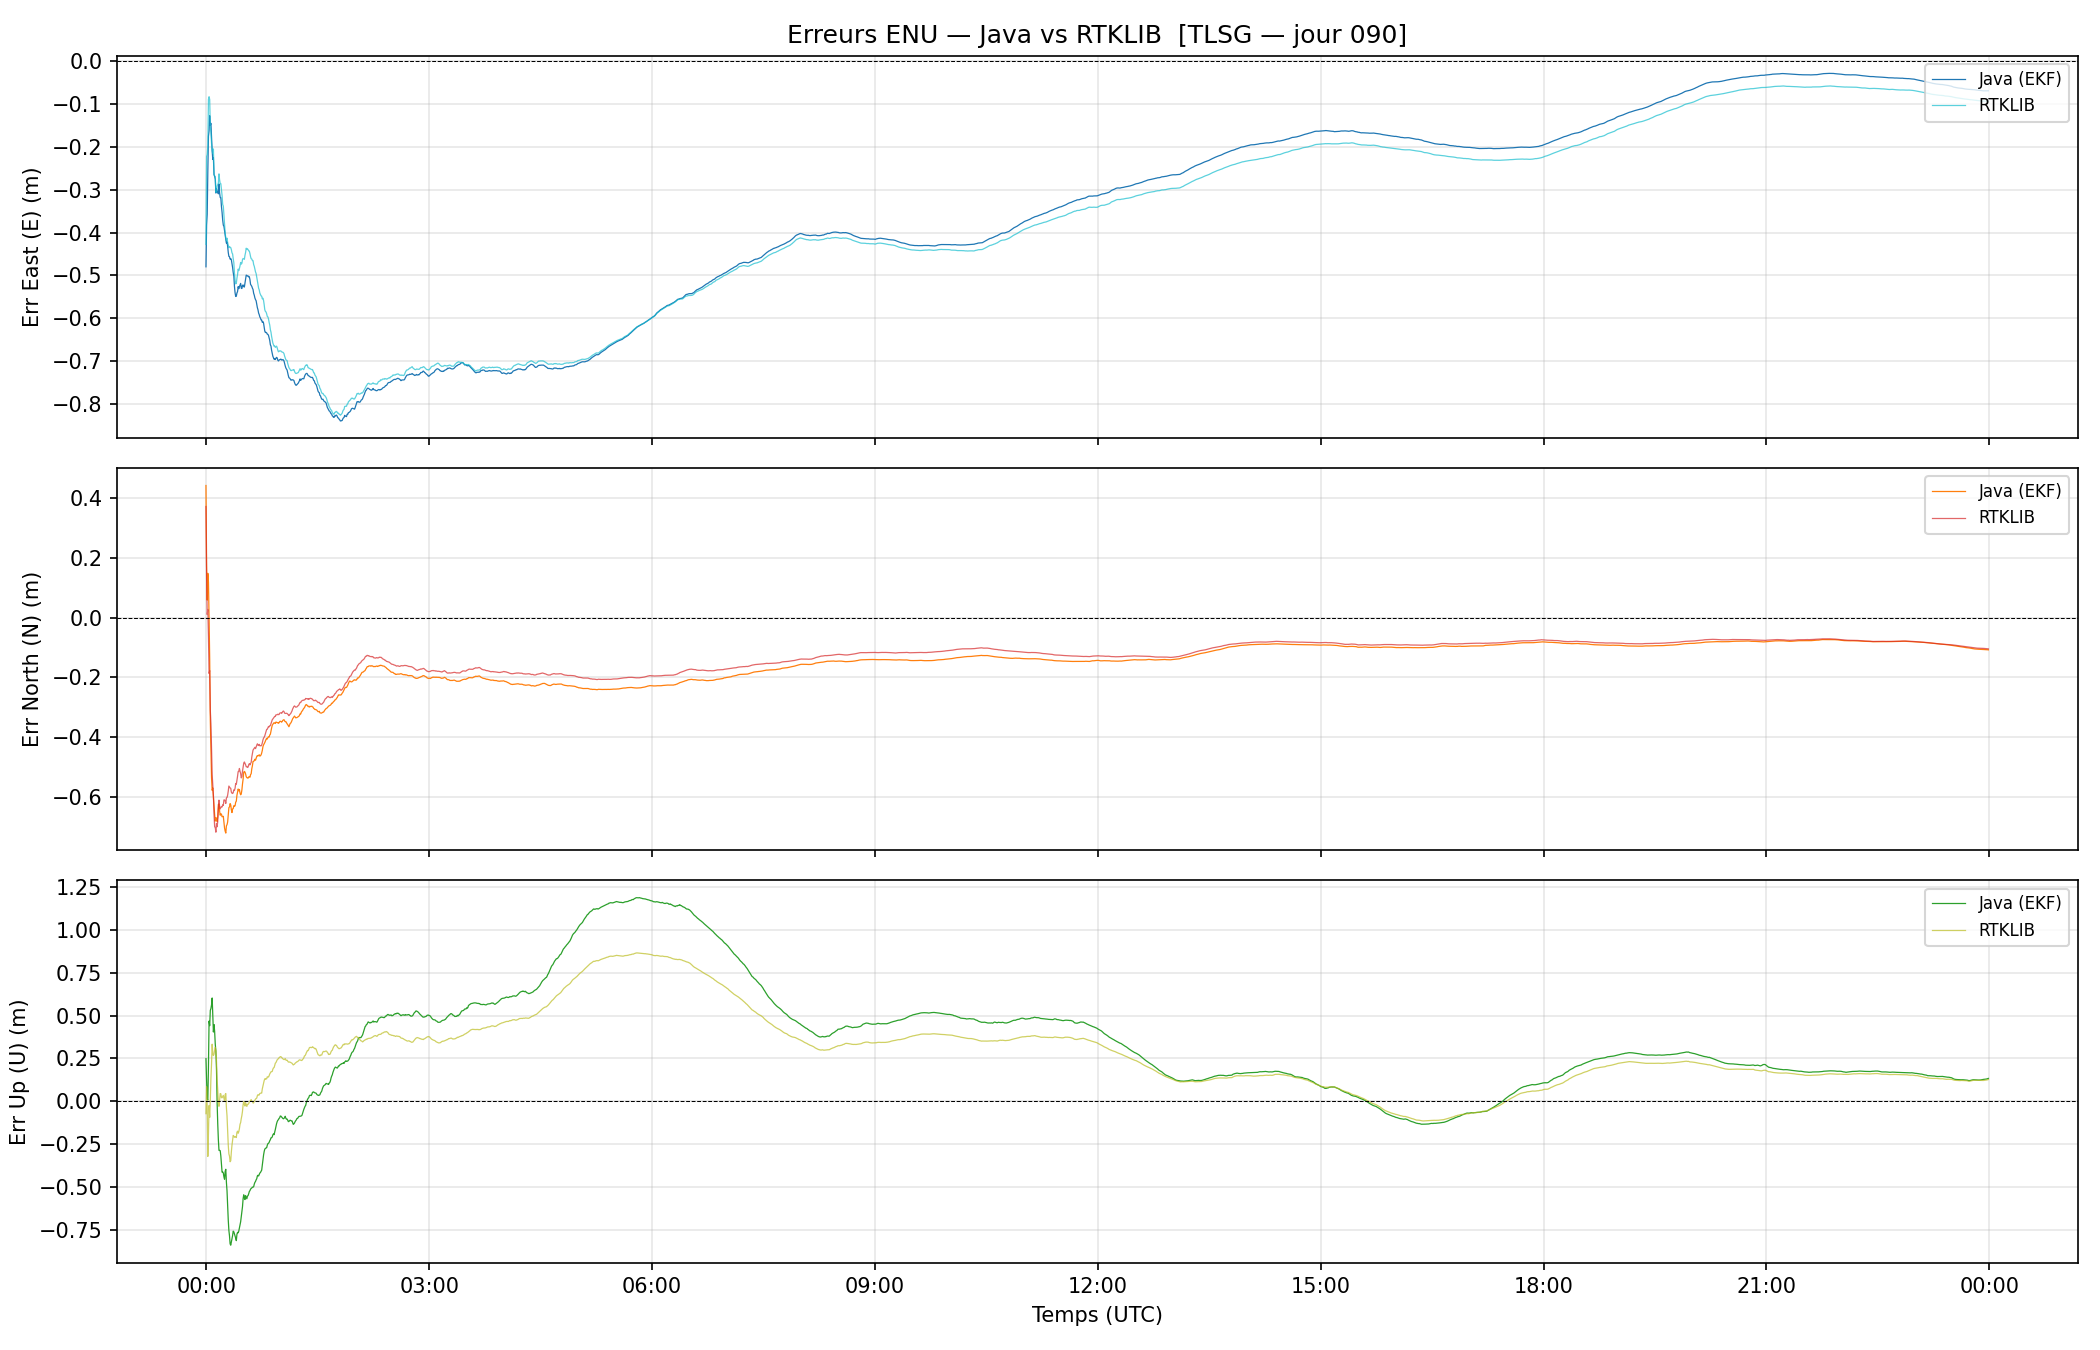
\includegraphics[width=\linewidth]{images/chapter5/ch5_ekf_tlsg_j090_gps_if_ztdgrad_broadcast_enu.png}
    \end{minipage}}
    \caption{Évolution des erreurs ENU pour les deux traitements
    troposphériques de l'EKF diffusé.}
    \label{fig:ch5_ekf_tropo_enu}
\end{figure}

L'estimation du ZTD et des gradients permet en principe d'absorber les
variations troposphériques qui ne sont pas représentées par SAAS. Elle ajoute
toutefois trois inconnues corrélées à la hauteur et nécessite une géométrie
suffisante pour les séparer. Dans ce cas, la RMSE 2D Java--Orekit varie peu
($0{,}461$~m avec SAAS et $0{,}464$~m avec ZTD+GRAD). Le retard troposphérique
agit principalement dans la direction verticale : l'estimation du ZTD et des
gradients doit donc surtout améliorer la composante Up lorsque ces paramètres
sont suffisamment observables. Sur ce cas, l'amélioration attendue n'est
toutefois pas obtenue. La RMSE Up Java--Orekit passe de $0{,}263$ à $0{,}480$~m
et celle de RTKLIB de $0{,}176$ à $0{,}359$~m ; la RMSE 3D augmente en
conséquence de $0{,}531$ à $0{,}668$~m côté Java--Orekit. Les courbes ENU
montrent que les composantes Est et Nord changent peu et que la différence se
concentre effectivement sur Up. L'ajout de paramètres troposphériques, plus
fortement corrélés à la hauteur, ne suffit donc pas à améliorer la solution
avec les seules éphémérides diffusées.

Les trajectoires horizontales Java--Orekit et RTKLIB ont la même forme pour les
deux modèles troposphériques. L'écart le plus important apparaît sur la
composante verticale de E-GRAD ; il indique une différence résiduelle dans la
pondération ou la dynamique des paramètres troposphériques, sans remettre en
cause la reproduction de la trajectoire horizontale. La comparaison ENU
montre également que les deux logiciels reproduisent la même évolution
temporelle dans chacun des deux modèles.


\section{Validation du traitement PPP précis}
\label{sec:validation_ppp_precise}

Le dernier essai conserve l'EKF, les observables, les constellations et le
traitement ZTD+GRAD de E-GRAD. Les éphémérides diffusées sont remplacées par les
produits précis SP3, CLK et BIA ; les marées solides, les corrections d'antenne
et le wind-up sont également activés. La comparaison porte donc sur le passage
du traitement diffusé au bloc PPP précis complet. La
figure~\ref{fig:ch5_ppp_precise_comparison} compare les nuages et la
figure~\ref{fig:ch5_ppp_precise_cdf} leurs distributions cumulées.

\begin{figure}[H]
    \centering
    \begin{minipage}[t]{0.48\textwidth}
        \centering
        \textbf{Référence E-GRAD : diffusées}\par\medskip
        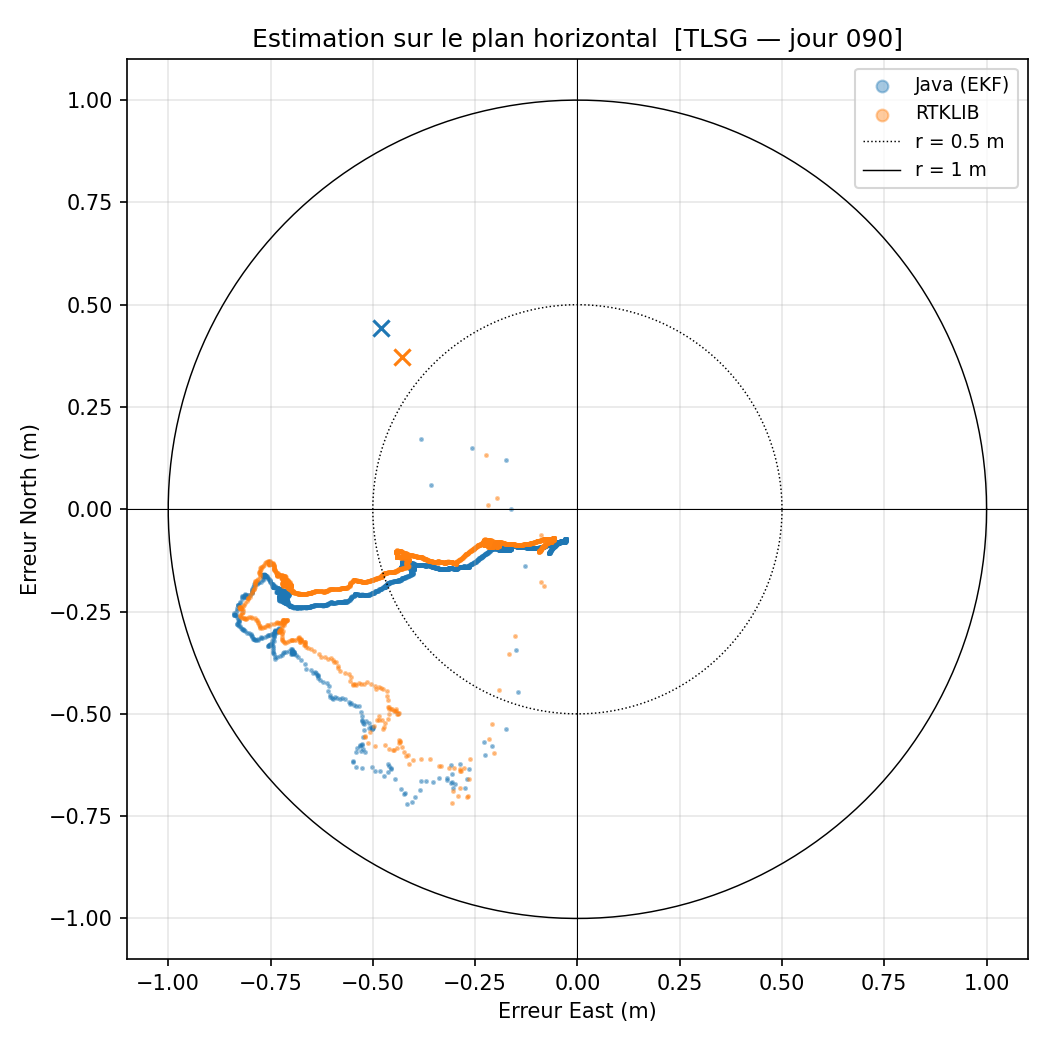
\includegraphics[width=\linewidth]{images/chapter5/ch5_ekf_tlsg_j090_gps_if_ztdgrad_broadcast_scatter_en.png}
    \end{minipage}
    \hfill
    \begin{minipage}[t]{0.48\textwidth}
        \centering
        \textbf{PPP : précises}\par\medskip
        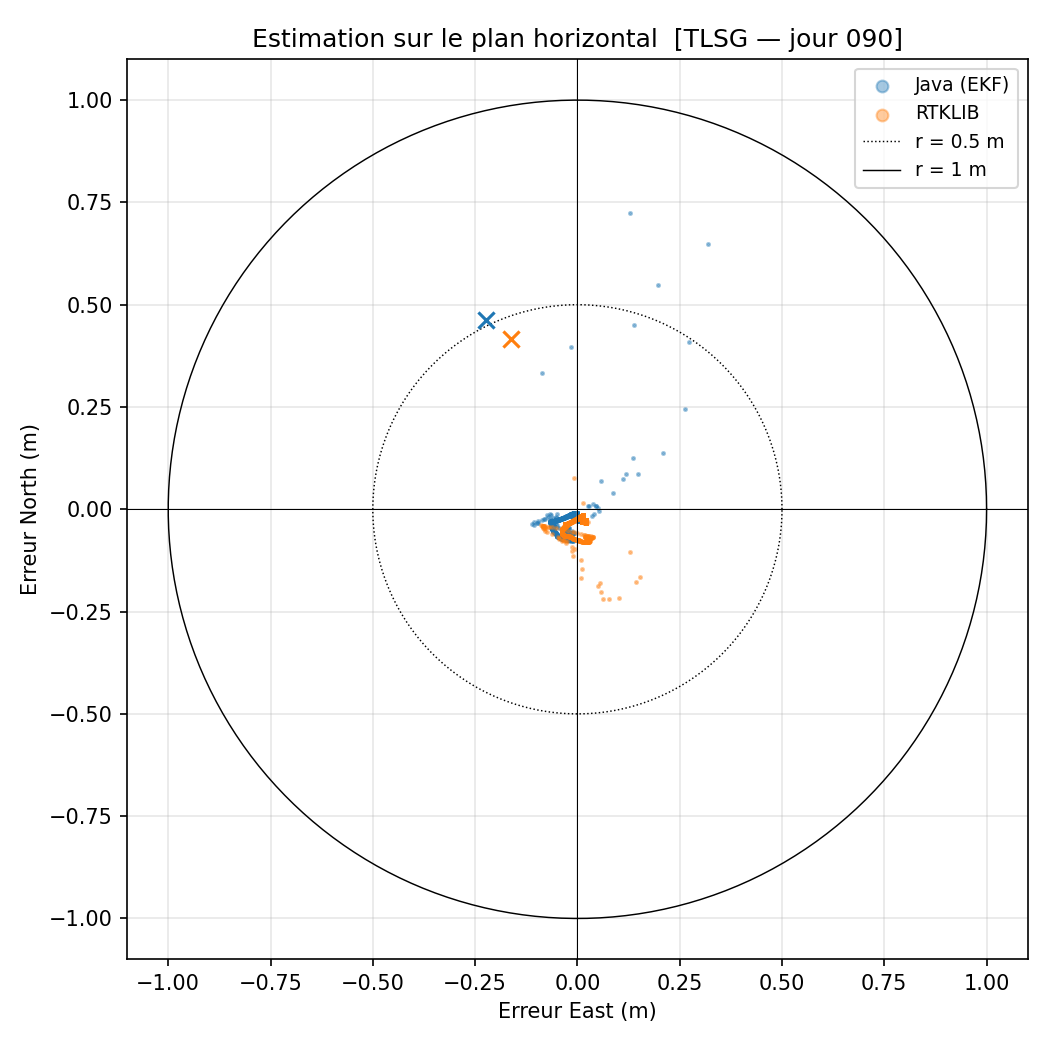
\includegraphics[width=\linewidth]{images/chapter5/ch5_ppp_tlsg_j090_gps_if_ztdgrad_precise_scatter_en.png}
    \end{minipage}
    \caption{Effet du passage aux produits et corrections PPP précis.}
    \label{fig:ch5_ppp_precise_comparison}
\end{figure}

\begin{figure}[H]
    \centering
    \makebox[\textwidth][c]{%
    \begin{minipage}[t]{0.64\textwidth}
        \centering
        \textbf{Référence E-GRAD : diffusées}\par\medskip
        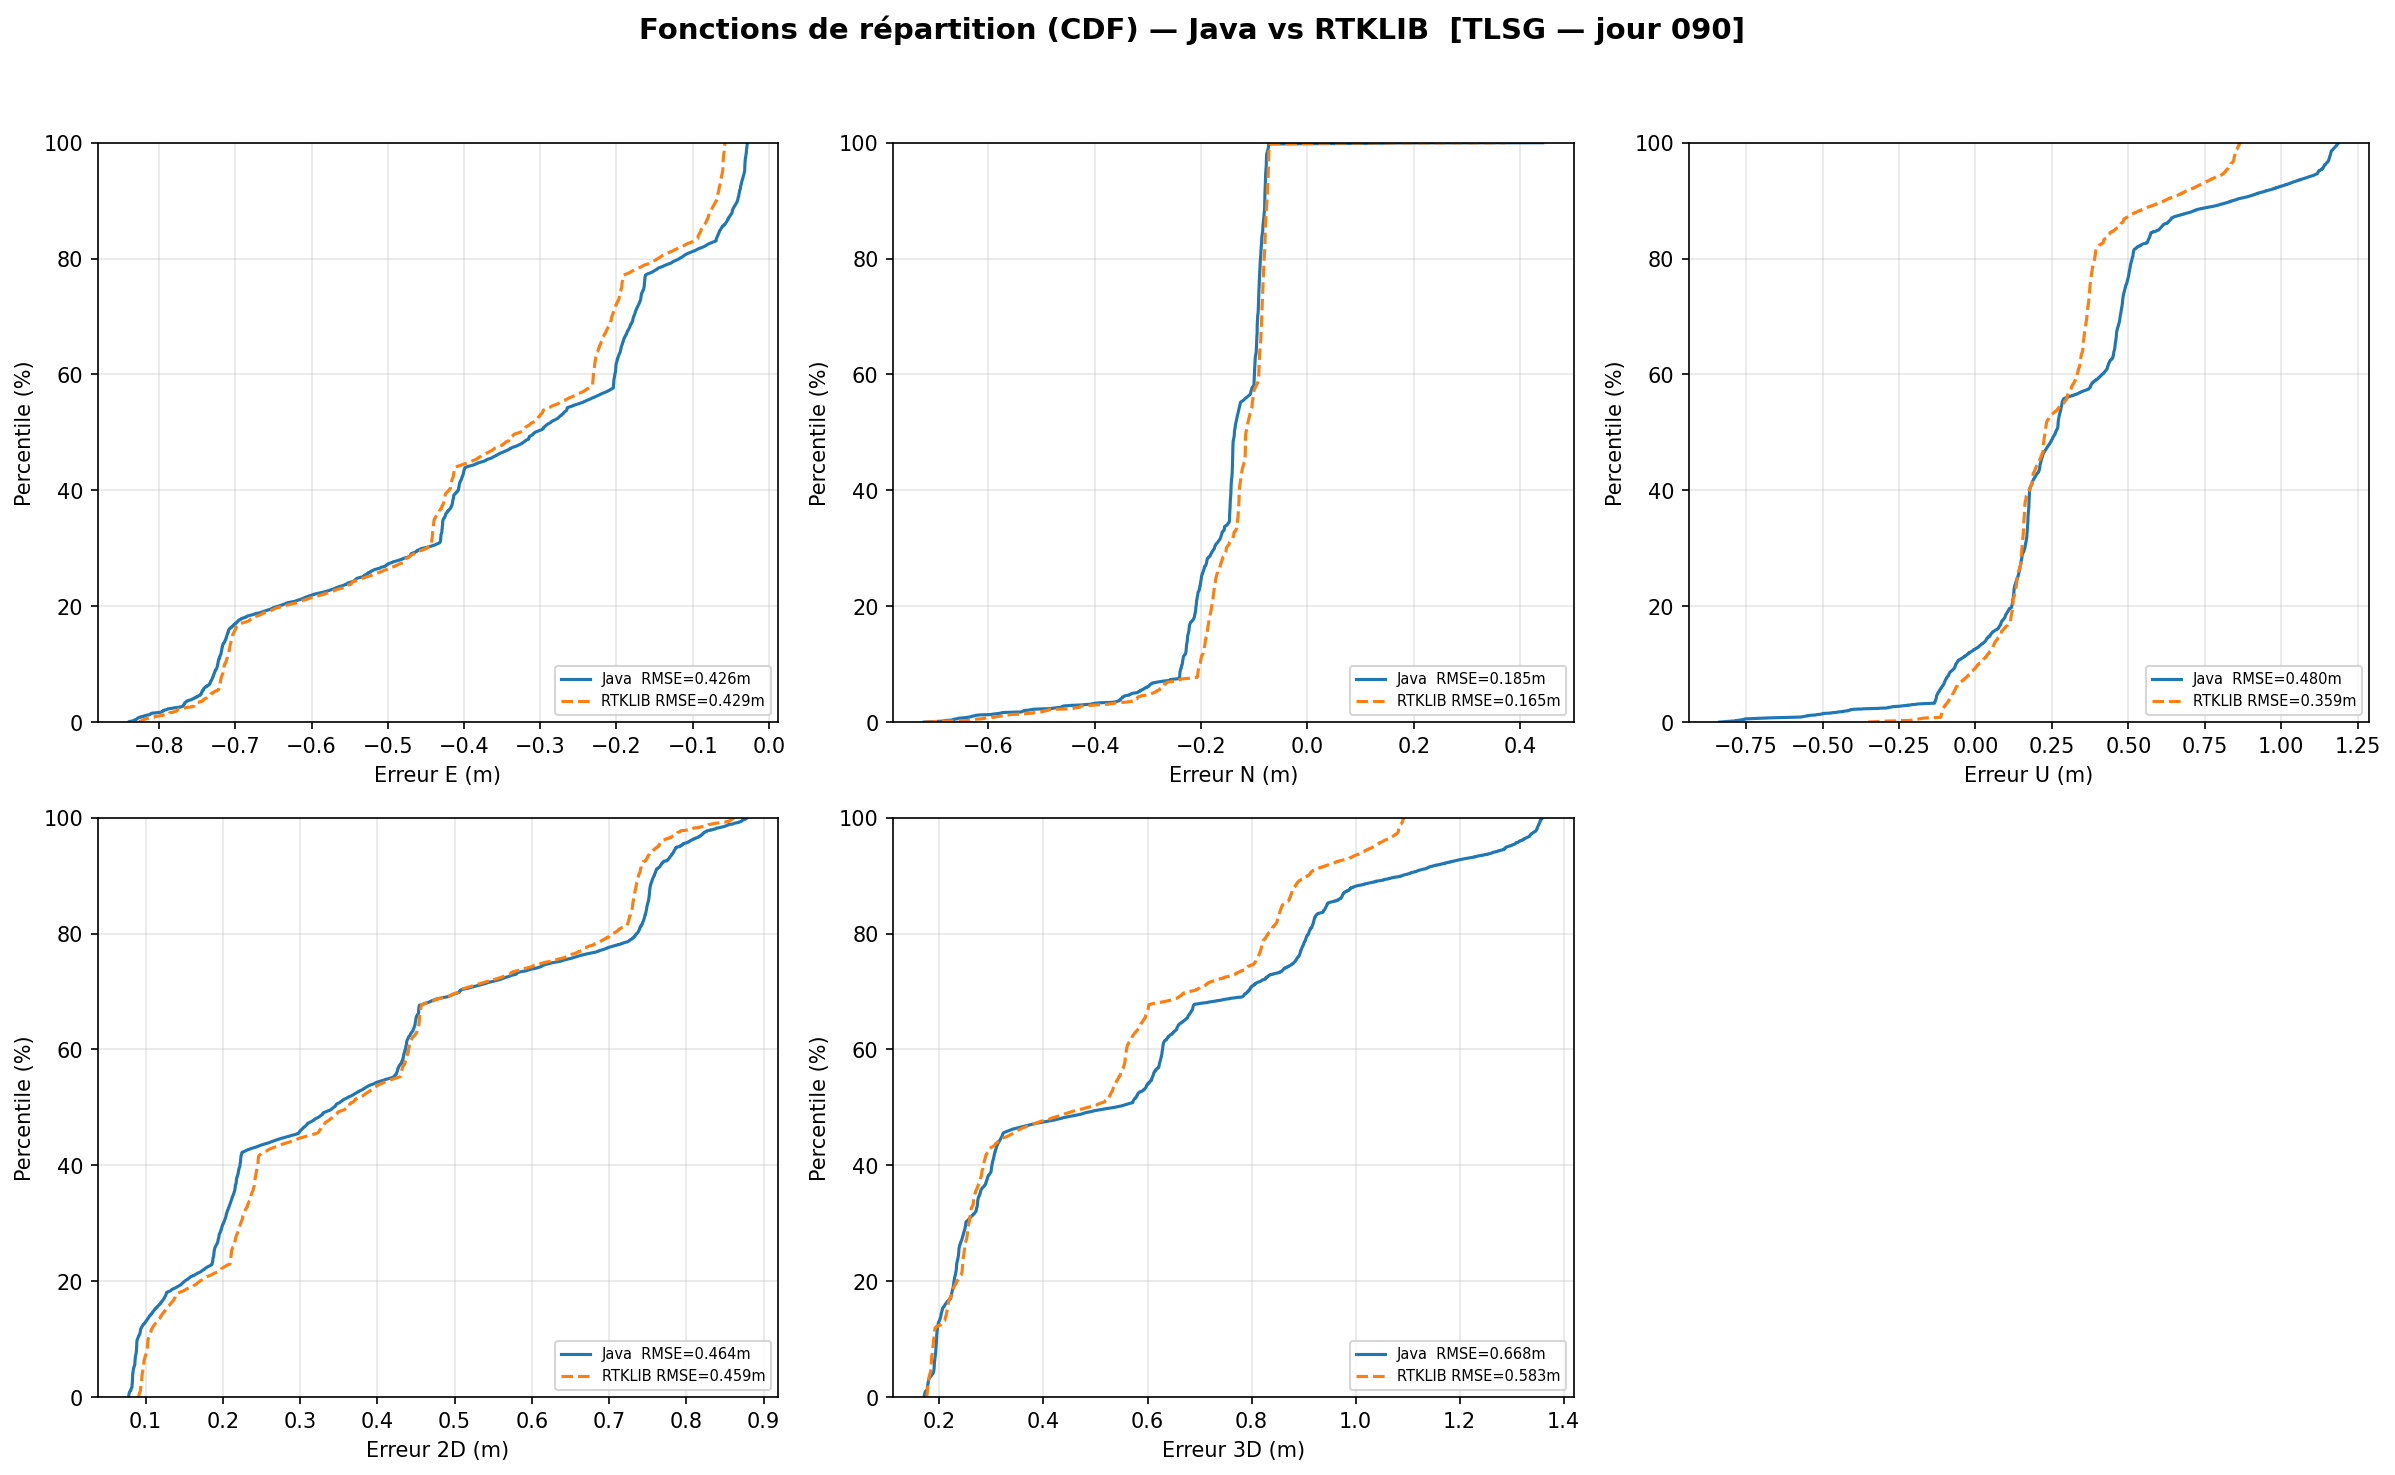
\includegraphics[width=\linewidth]{images/chapter5/ch5_ekf_tlsg_j090_gps_if_ztdgrad_broadcast_cdf.png}
    \end{minipage}
    \hspace{0.01\textwidth}
    \begin{minipage}[t]{0.64\textwidth}
        \centering
        \textbf{PPP : précises}\par\medskip
        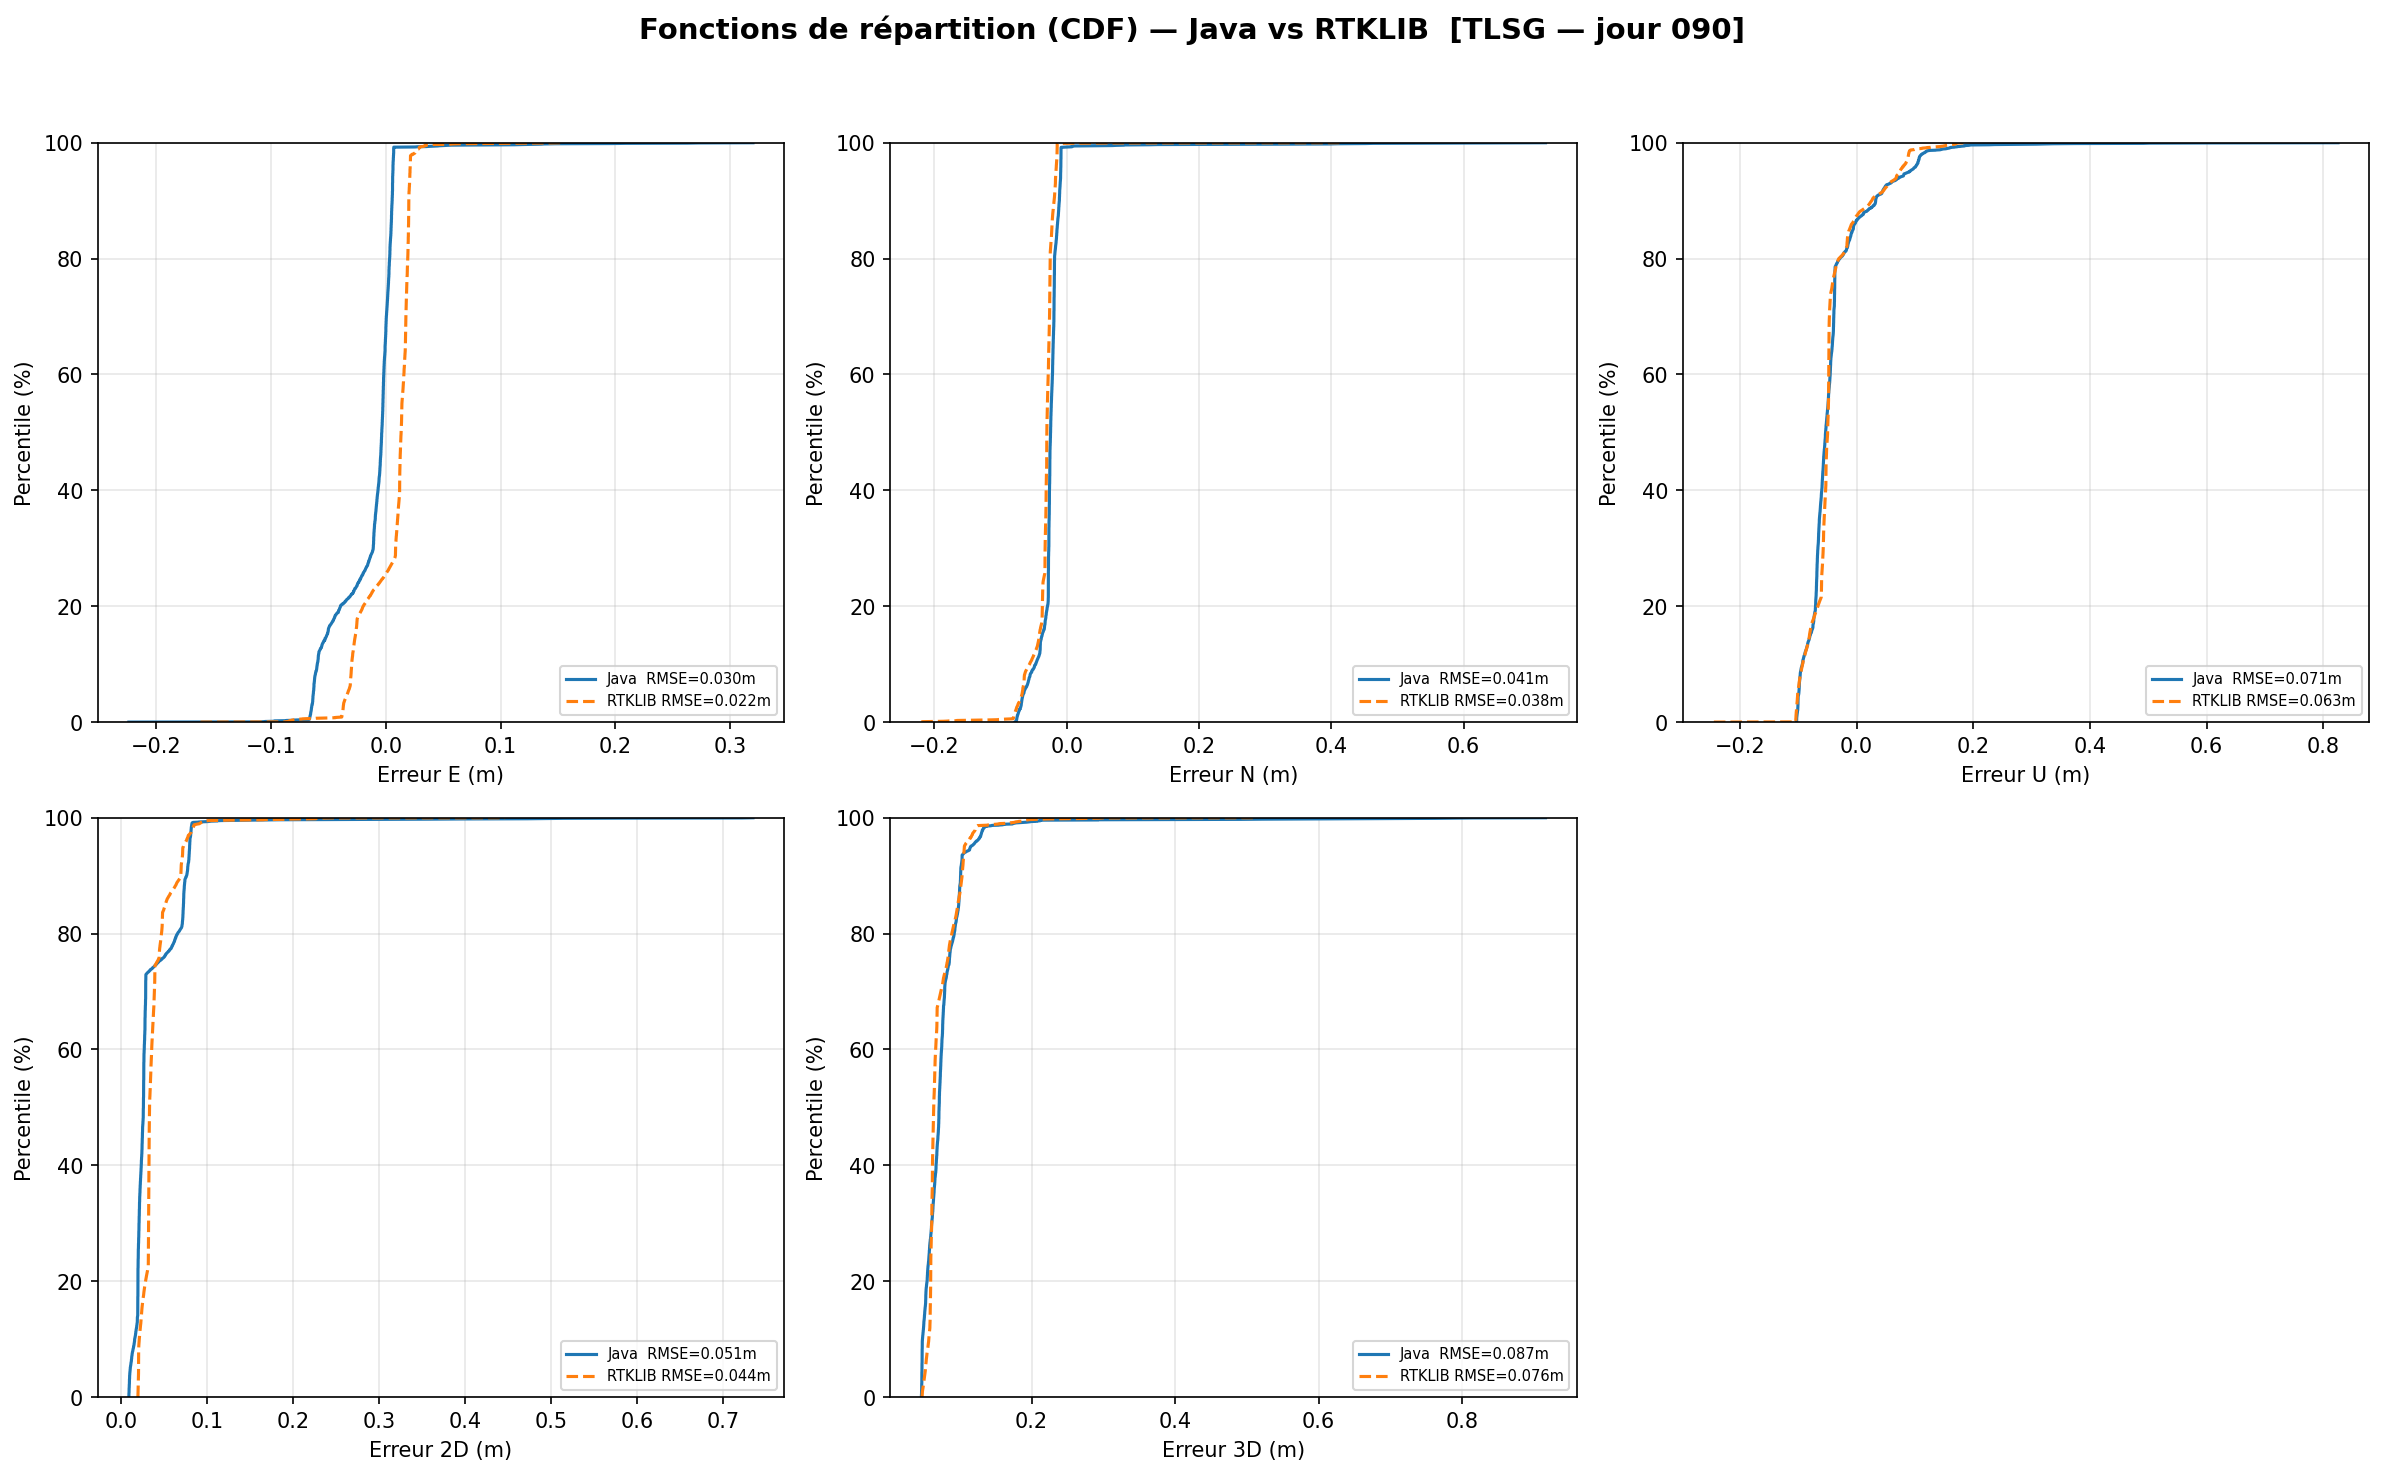
\includegraphics[width=\linewidth]{images/chapter5/ch5_ppp_tlsg_j090_gps_if_ztdgrad_precise_cdf.png}
    \end{minipage}}
    \caption{Fonctions de répartition des erreurs avant et après le passage
    aux produits et corrections PPP précis.}
    \label{fig:ch5_ppp_precise_cdf}
\end{figure}

La réduction de l'incertitude sur les orbites et les horloges, associée aux
corrections fines, diminue fortement l'erreur. La RMSE 2D Java--Orekit passe de
$0{,}464$~m à $0{,}051$~m et la RMSE 3D de $0{,}668$ à $0{,}087$~m. RTKLIB
présente la même amélioration, avec respectivement $0{,}044$ et $0{,}076$~m
dans la configuration précise. La majorité des estimations est concentrée à
quelques centimètres de la position vraie. Les deux chaînes convergent vers la
même zone, même si quelques points Java--Orekit isolés pendant l'initialisation
produisent une dispersion légèrement supérieure. Le déplacement très net des
CDF vers zéro montre que ce gain concerne la quasi-totalité des époques et ne
résulte pas seulement de quelques estimations particulièrement précises.


\subsection{Convergence et covariance formelle}

La figure~\ref{fig:ch5_ppp_enu} détaille la convergence du traitement précis.
Le transitoire des premières minutes correspond à l'initialisation du filtre et
des ambiguïtés. Après cette phase, les composantes Nord et Vertical des deux
solutions sont très proches. Un écart Est de quelques centimètres subsiste
pendant une partie de la journée, puis diminue.

\begin{figure}[H]
    \centering
    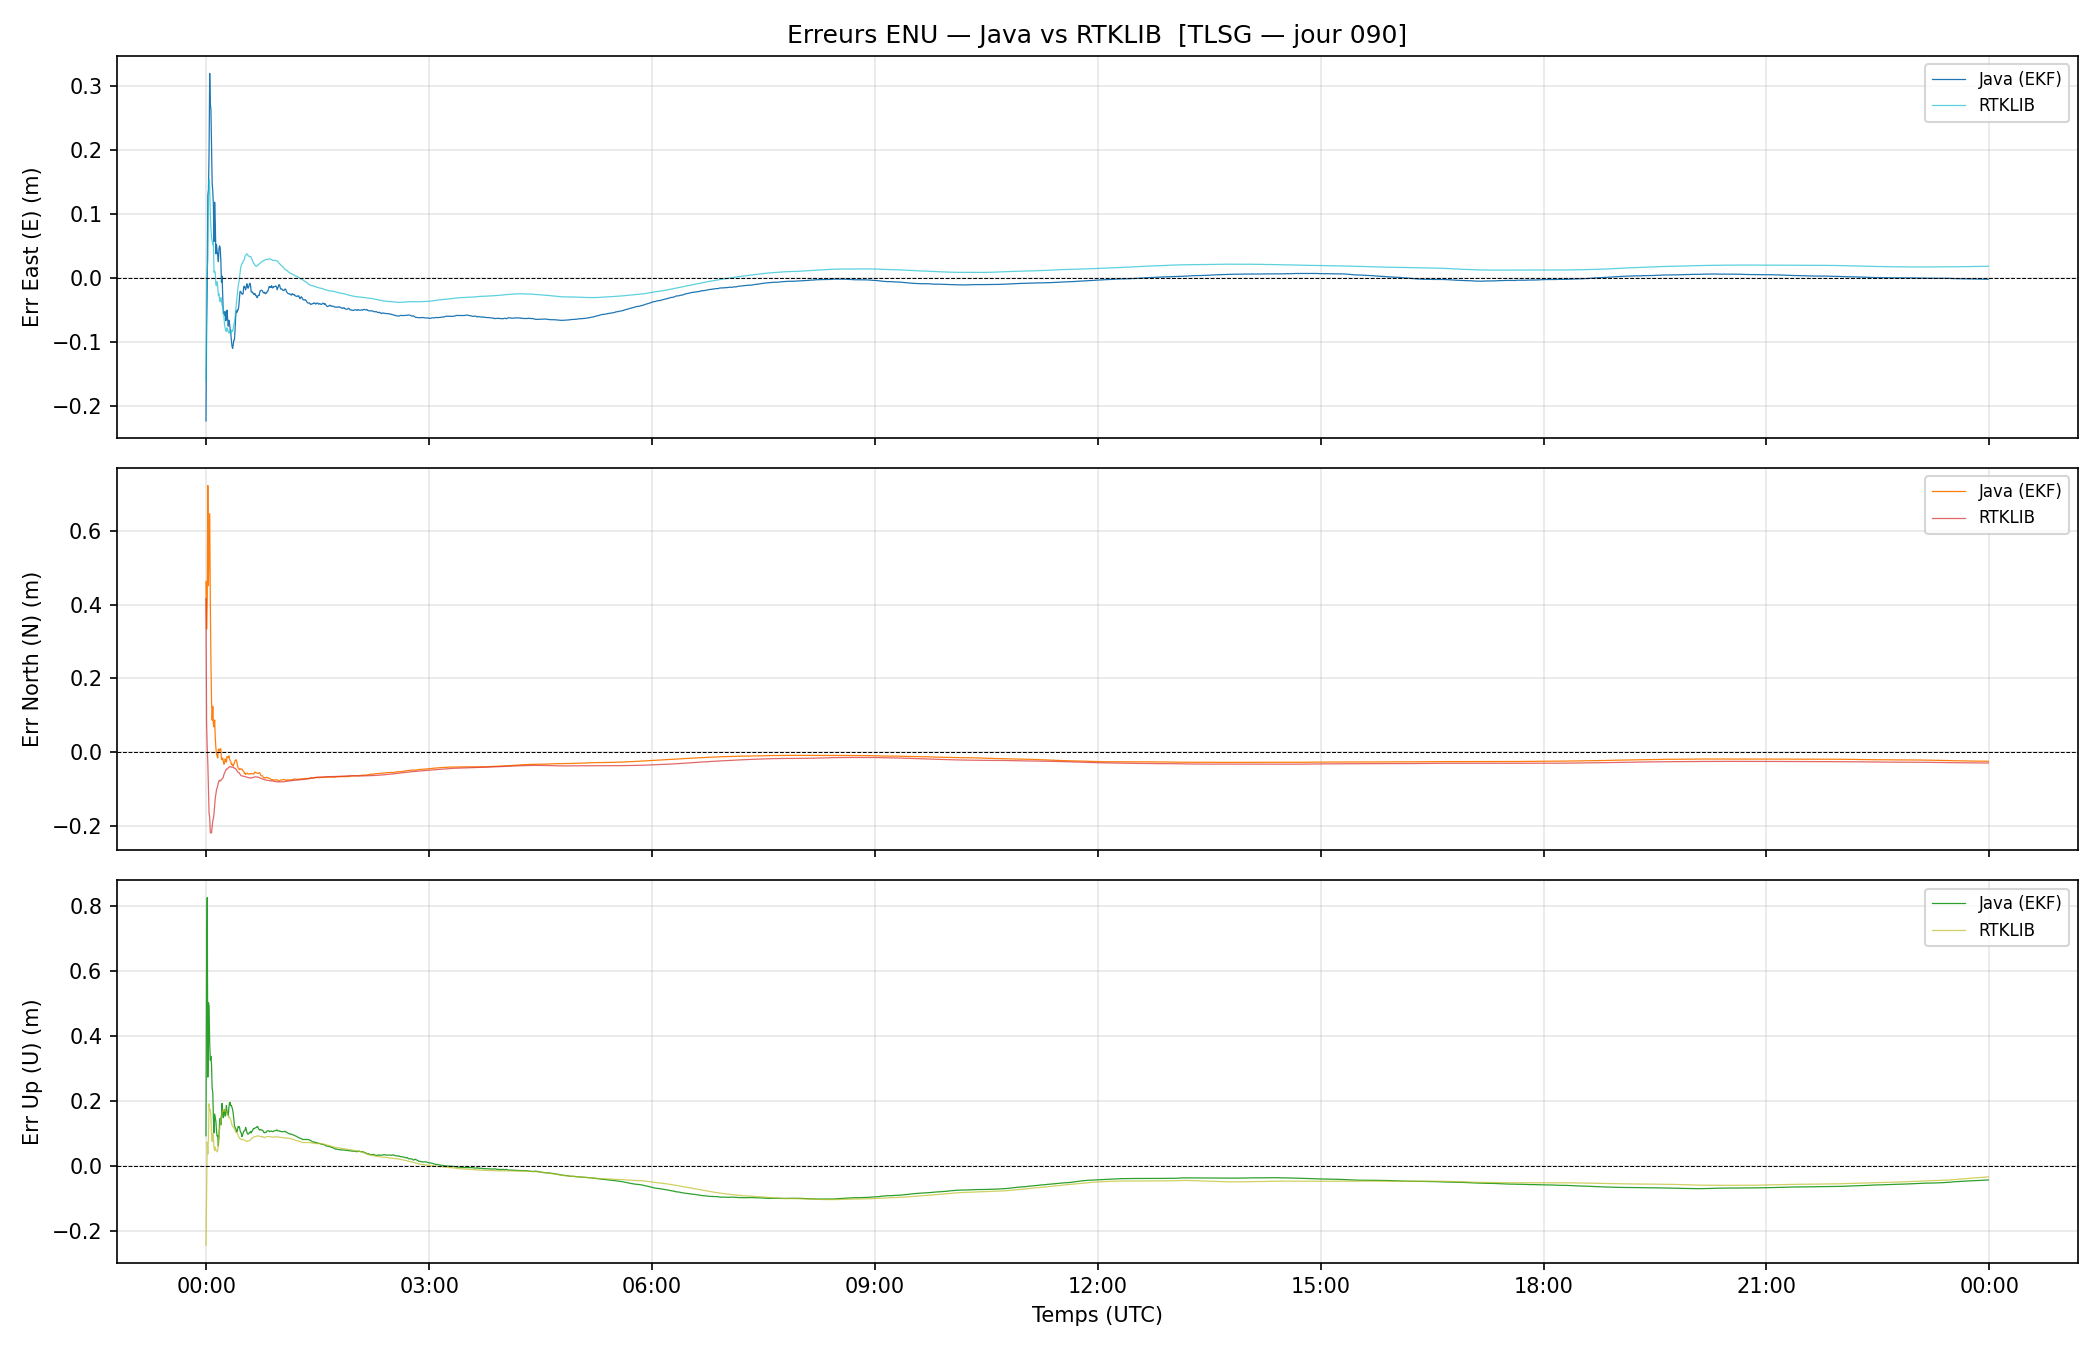
\includegraphics[width=\textwidth]{images/chapter5/ch5_ppp_tlsg_j090_gps_if_ztdgrad_precise_enu.png}
    \caption{Évolution des erreurs ENU du traitement PPP précis.}
    \label{fig:ch5_ppp_enu}
\end{figure}

Les écarts-types formels de la figure~\ref{fig:ch5_ppp_sigma} décroissent
rapidement après l'initialisation. Les deux filtres suivent la même dynamique
et atteignent des incertitudes millimétriques dans le plan horizontal. La
variance verticale Java--Orekit devient plus faible que celle de RTKLIB après
la phase initiale. Cette observation ne signifie pas que l'erreur verticale
réelle est plus faible : la covariance formelle caractérise le modèle
stochastique du filtre et doit être confrontée aux erreurs observées.

\begin{figure}[H]
    \centering
    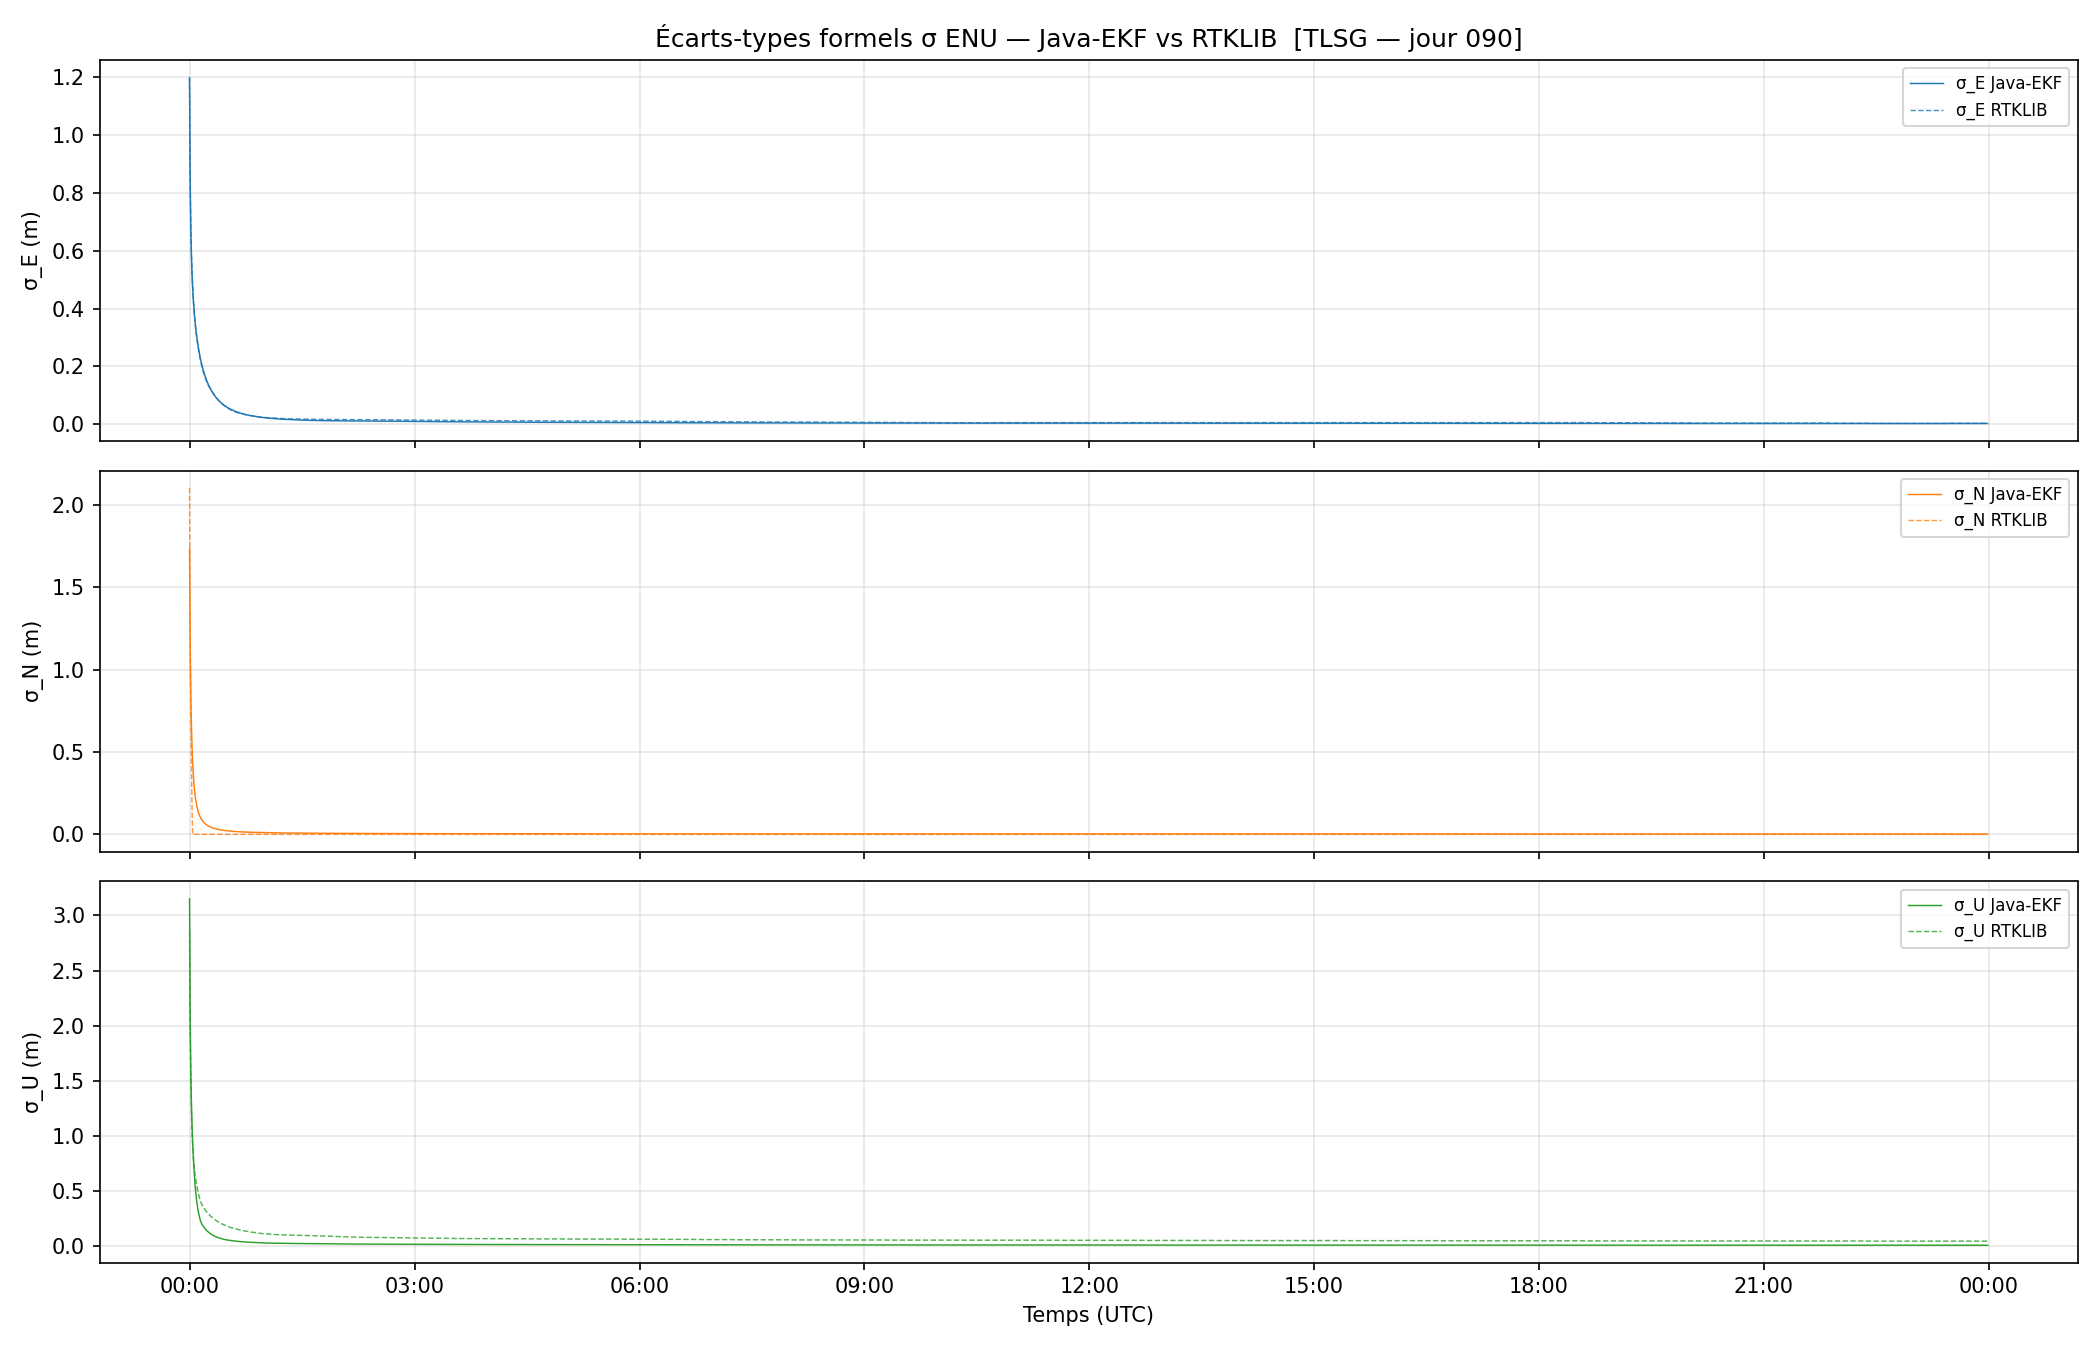
\includegraphics[width=\textwidth]{images/chapter5/ch5_ppp_tlsg_j090_gps_if_ztdgrad_precise_sigma.png}
    \caption{Écarts-types formels des composantes ENU du traitement PPP
    précis.}
    \label{fig:ch5_ppp_sigma}
\end{figure}


\subsection{Paramètres troposphériques}

La figure~\ref{fig:ch5_ppp_tropo} compare les paramètres estimés à ceux de
RTKLIB et au produit troposphérique IGS. Le ZTD Java--Orekit suit la même
évolution générale que RTKLIB, mais les amplitudes diffèrent de plusieurs
centimètres et les deux séries s'écartent du produit IGS sur certaines plages.
Les gradients présentent des différences plus marquées : leurs variations
lentes sont comparables, mais ni leur amplitude ni leur phase ne coïncident
exactement, tandis que le produit IGS reste plus proche de zéro.

Ces écarts ne se reportent pas intégralement sur la position, car le ZTD, les
gradients, l'horloge et les ambiguïtés sont corrélés dans l'estimation. La bonne
superposition des coordonnées ne suffit donc pas à valider séparément chaque
paramètre de nuisance. La troposphère constitue ici la principale limite de la
reproduction et nécessite une validation dédiée des conventions, des
contraintes stochastiques et des fonctions de projection.

\begin{figure}[H]
    \centering
    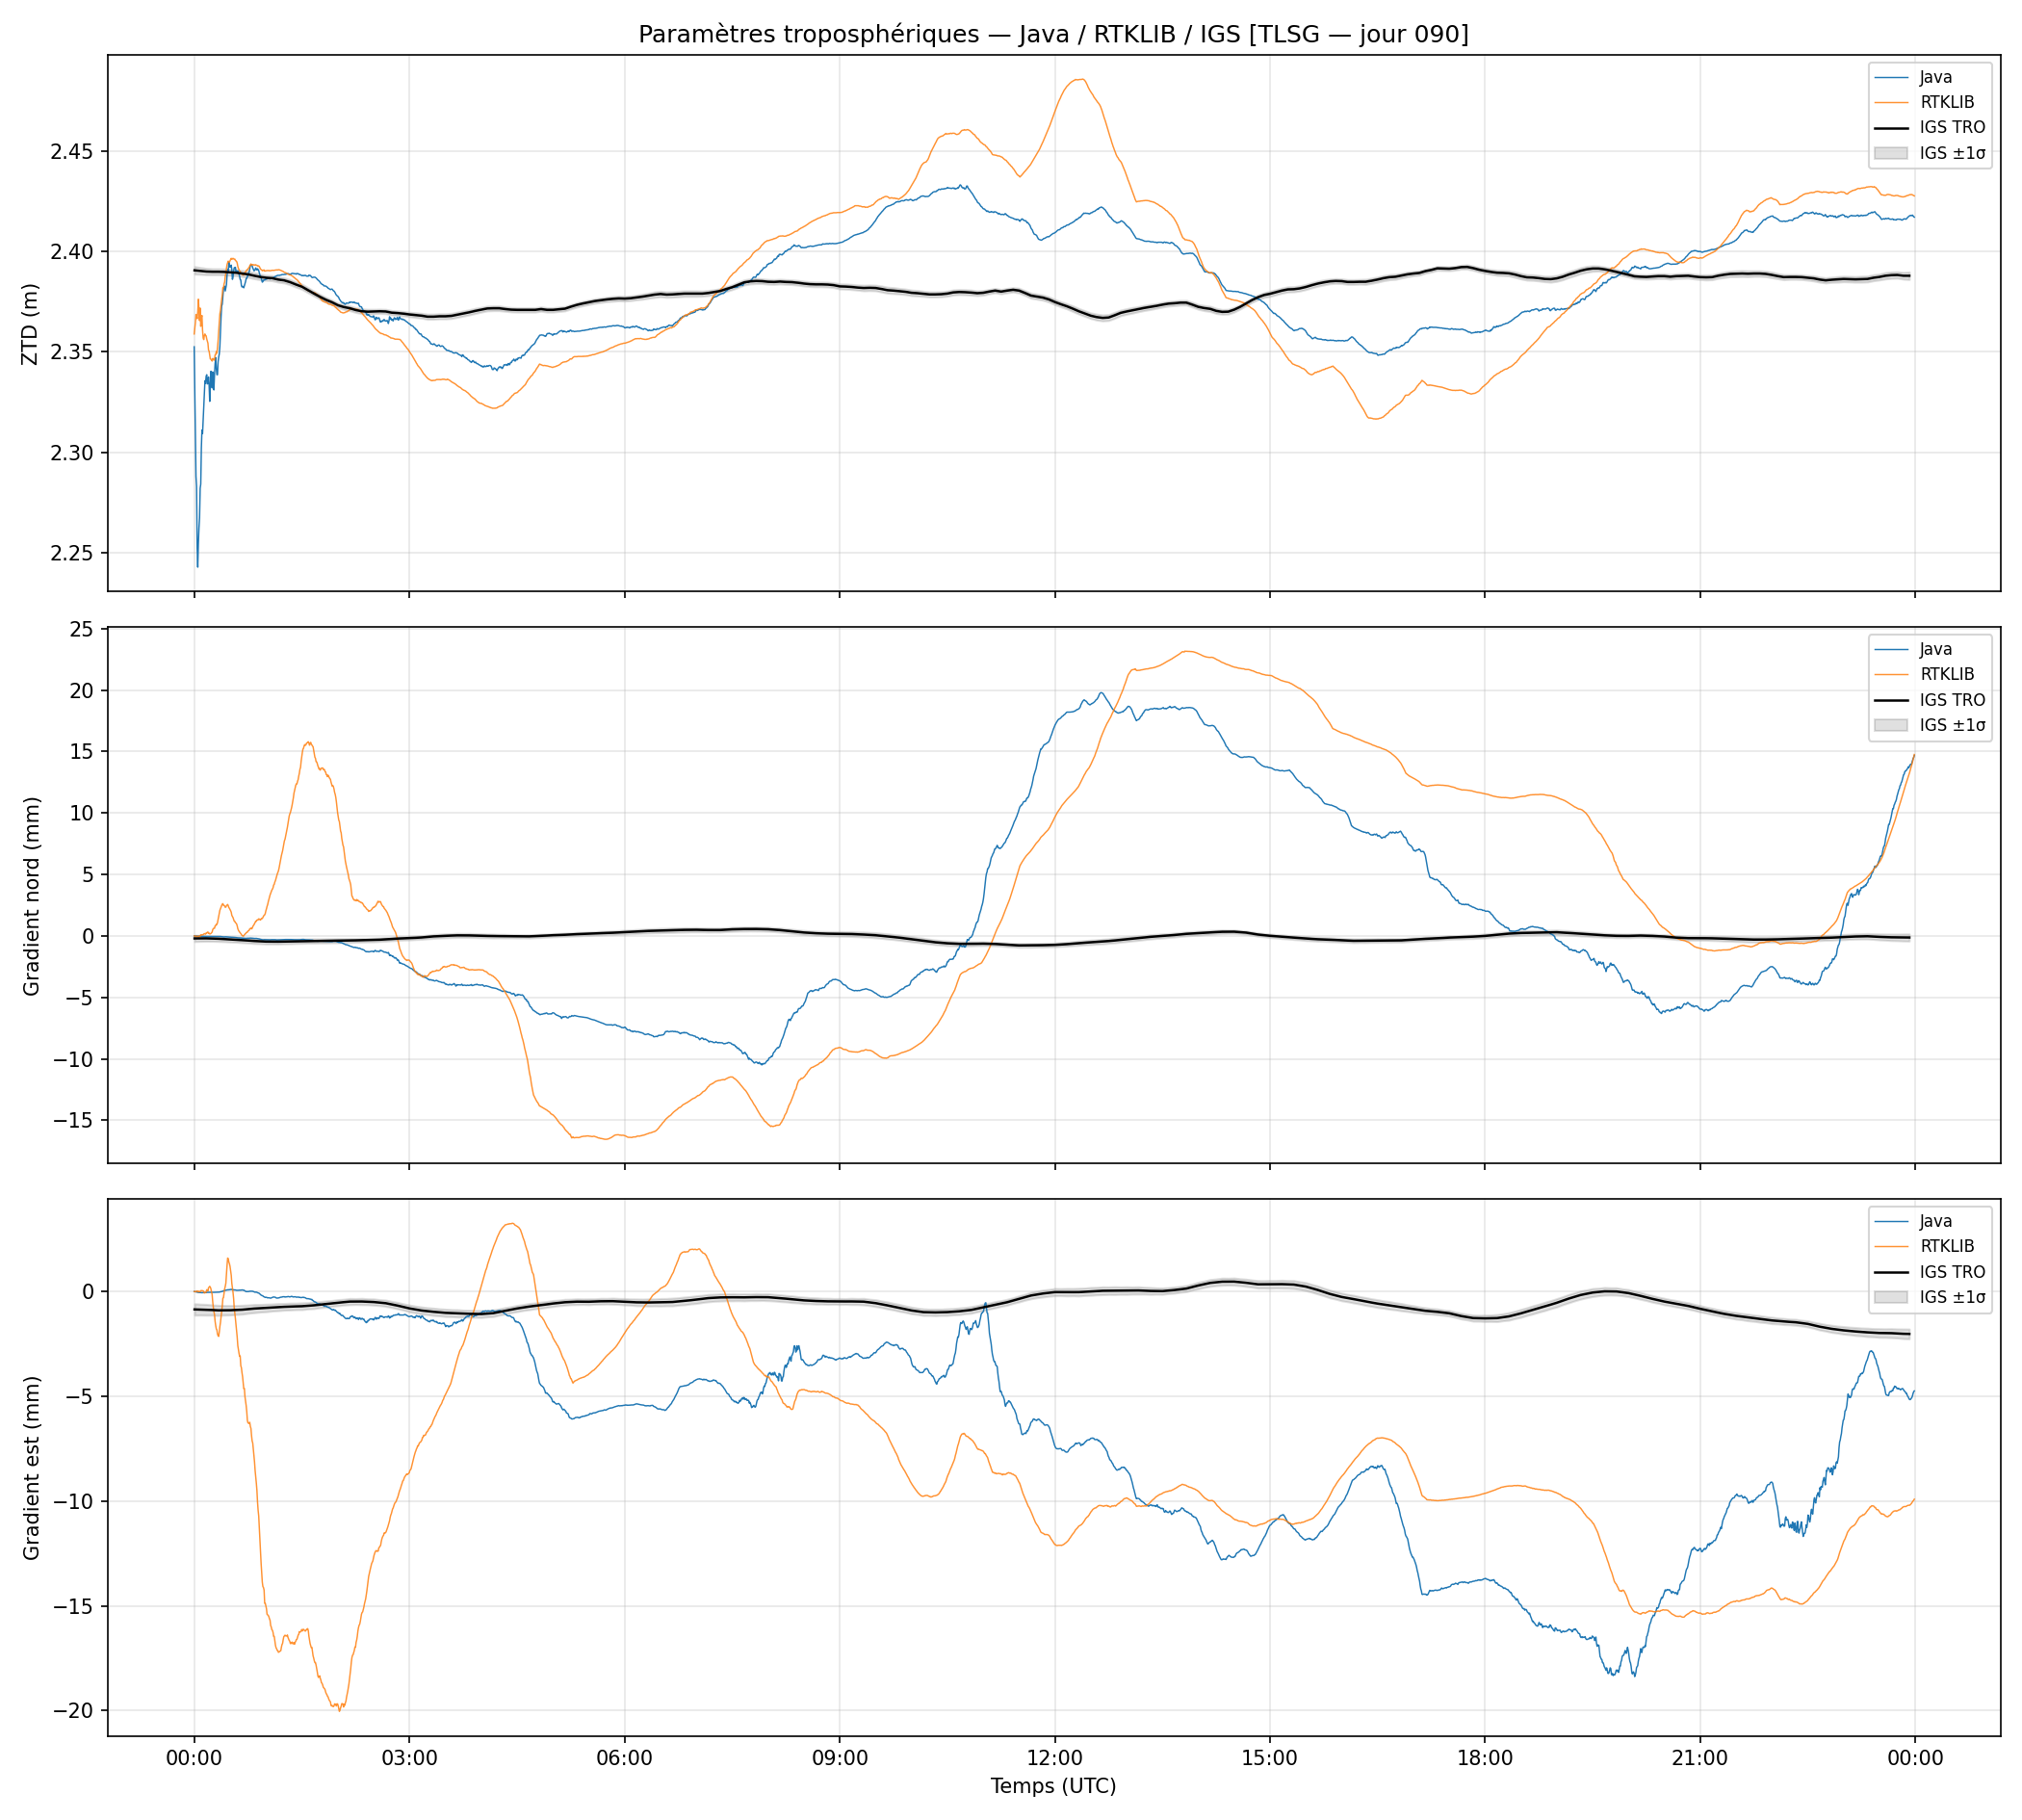
\includegraphics[width=\textwidth]{images/chapter5/ch5_ppp_tlsg_j090_gps_if_ztdgrad_precise_tropo.png}
    \caption{ZTD et gradients troposphériques du traitement PPP précis. Le
    produit IGS est représenté avec son intervalle formel à $1\sigma$.}
    \label{fig:ch5_ppp_tropo}
\end{figure}


\section{Synthèse}
\label{sec:validation_synthesis}

Le tableau~\ref{tab:validation_rmse} rassemble les RMSE des sept
configurations. Il permet de distinguer l'effet physique du paramètre modifié
de l'écart entre les deux implémentations.

\begin{table}[H]
\centering
\caption{RMSE horizontales et tridimensionnelles des configurations
représentatives.}
\label{tab:validation_rmse}
\small
\begin{tabular}{lrrrr}
\hline
& \multicolumn{2}{c}{\textbf{RMSE 2D (m)}} &
  \multicolumn{2}{c}{\textbf{RMSE 3D (m)}} \\
\textbf{Cas} & \textbf{Java--Orekit} & \textbf{RTKLIB} &
\textbf{Java--Orekit} & \textbf{RTKLIB} \\
\hline
S-REF  & 1,252 & 1,212 & 2,927 & 2,764 \\
S-YEBE & 1,373 & 1,365 & 2,825 & 2,802 \\
S-GAL  & 0,832 & 0,774 & 1,839 & 1,676 \\
S-KLO  & 0,860 & 0,859 & 2,236 & 2,292 \\
E-REF  & 0,461 & 0,459 & 0,531 & 0,492 \\
E-GRAD & 0,464 & 0,459 & 0,668 & 0,583 \\
PPP    & 0,051 & 0,044 & 0,087 & 0,076 \\
\hline
\end{tabular}
\end{table}

La comparaison paramètre par paramètre conduit à trois résultats. Premièrement,
le mode Single reproduit RTKLIB pour les deux stations, les deux traitements
ionosphériques et la configuration GPS+Galileo. Deuxièmement, l'ajout de
Galileo réduit nettement la dispersion, tandis que l'effet du choix IF ou KLO
dépend du compromis entre erreur de modèle et amplification du bruit.
Troisièmement, l'estimation troposphérique seule n'améliore pas le cas diffusé,
mais le traitement PPP complet abaisse l'erreur du mètre au centimètre.

Les résultats présentés correspondent au jour 090. Les campagnes couvrant les
jours 090 et 137 ainsi que TLSG et YEBE restent nécessaires pour vérifier que
ces conclusions ne dépendent pas d'une géométrie ou de conditions
atmosphériques particulières.
